\documentclass[11pt,]{article}
\usepackage[left=1in,top=1in,right=1in,bottom=1in]{geometry}
\newcommand*{\authorfont}{\fontfamily{phv}\selectfont}
\usepackage[]{mathpazo}


  \usepackage[T1]{fontenc}
  \usepackage[utf8]{inputenc}



\usepackage{abstract}
\renewcommand{\abstractname}{}    % clear the title
\renewcommand{\absnamepos}{empty} % originally center

\renewenvironment{abstract}
 {{%
    \setlength{\leftmargin}{0mm}
    \setlength{\rightmargin}{\leftmargin}%
  }%
  \relax}
 {\endlist}

\makeatletter
\def\@maketitle{%
  \newpage
%  \null
%  \vskip 2em%
%  \begin{center}%
  \let \footnote \thanks
    {\fontsize{18}{20}\selectfont\raggedright  \setlength{\parindent}{0pt} \@title \par}%
}
%\fi
\makeatother




\setcounter{secnumdepth}{3}

\usepackage{longtable,booktabs}

\usepackage{graphicx,grffile}
\makeatletter
\def\maxwidth{\ifdim\Gin@nat@width>\linewidth\linewidth\else\Gin@nat@width\fi}
\def\maxheight{\ifdim\Gin@nat@height>\textheight\textheight\else\Gin@nat@height\fi}
\makeatother
% Scale images if necessary, so that they will not overflow the page
% margins by default, and it is still possible to overwrite the defaults
% using explicit options in \includegraphics[width, height, ...]{}
\setkeys{Gin}{width=\maxwidth,height=\maxheight,keepaspectratio}

\title{Diversidad, ecología espacial y ordenación de la familia Euphorbeaceae
en Isla Barro Colorado, Panama (2010)\\[2\baselineskip]Subtítulo  }



\author{\Large Yeiny Pamela Reyes Z.\vspace{0.05in} \newline\normalsize\emph{Estudiante, Universidad Autónoma de Santo Domingo (UASD)}  }


\date{}

\usepackage{titlesec}

\titleformat*{\section}{\normalsize\bfseries}
\titleformat*{\subsection}{\normalsize\itshape}
\titleformat*{\subsubsection}{\normalsize\itshape}
\titleformat*{\paragraph}{\normalsize\itshape}
\titleformat*{\subparagraph}{\normalsize\itshape}

\titlespacing{\section}
{0pt}{36pt}{0pt}
\titlespacing{\subsection}
{0pt}{36pt}{0pt}
\titlespacing{\subsubsection}
{0pt}{36pt}{0pt}





\newtheorem{hypothesis}{Hypothesis}
\usepackage{setspace}

\makeatletter
\@ifpackageloaded{hyperref}{}{%
\ifxetex
  \PassOptionsToPackage{hyphens}{url}\usepackage[setpagesize=false, % page size defined by xetex
              unicode=false, % unicode breaks when used with xetex
              xetex]{hyperref}
\else
  \PassOptionsToPackage{hyphens}{url}\usepackage[unicode=true]{hyperref}
\fi
}

\@ifpackageloaded{color}{
    \PassOptionsToPackage{usenames,dvipsnames}{color}
}{%
    \usepackage[usenames,dvipsnames]{color}
}
\makeatother
\hypersetup{breaklinks=true,
            bookmarks=true,
            pdfauthor={Yeiny Pamela Reyes Z. (Estudiante, Universidad Autónoma de Santo Domingo (UASD))},
             pdfkeywords = {Euphorbiaceae, Abundancia,diversidad,ordenación},  
            pdftitle={Diversidad, ecología espacial y ordenación de la familia Euphorbeaceae
en Isla Barro Colorado, Panama (2010)\\[2\baselineskip]Subtítulo},
            colorlinks=true,
            citecolor=blue,
            urlcolor=blue,
            linkcolor=magenta,
            pdfborder={0 0 0}}
\urlstyle{same}  % don't use monospace font for urls

% set default figure placement to htbp
\makeatletter
\def\fps@figure{htbp}
\makeatother

\usepackage{pdflscape} \newcommand{\blandscape}{\begin{landscape}}
\newcommand{\elandscape}{\end{landscape}}


% add tightlist ----------
\providecommand{\tightlist}{%
\setlength{\itemsep}{0pt}\setlength{\parskip}{0pt}}

\begin{document}
	
% \pagenumbering{arabic}% resets `page` counter to 1 
%
% \maketitle

{% \usefont{T1}{pnc}{m}{n}
\setlength{\parindent}{0pt}
\thispagestyle{plain}
{\fontsize{18}{20}\selectfont\raggedright 
\maketitle  % title \par  

}

{
   \vskip 13.5pt\relax \normalsize\fontsize{11}{12} 
\textbf{\authorfont Yeiny Pamela Reyes Z.} \hskip 15pt \emph{\small Estudiante, Universidad Autónoma de Santo Domingo (UASD)}   

}

}








\begin{abstract}

    \hbox{\vrule height .2pt width 39.14pc}

    \vskip 8.5pt % \small 

\noindent Los censos son una gran herramientas que pueden servir de insumo para
profundizar en estudios sobre la ecología de la comunidad, tales como:
asociación de variables ambientales y su relación con patrones
espaciales/temporales (e.g.~influencia de la edafología y la
geomorfología en la abundancia y distribución de especies),así como para
conocer y tratar de entender comportamientos de especies raras, entre
otros aspectos. . Es por eso que desde hace ya 40 años(referencia actual
2020) en Barro Colorado se inició un proyecto a cargo del Instituto
Smithsonian de Investigaciones Tropicales o STRI por sus siglas en
inglés, el cual consiste en un censo para estudiar la composición
florística del bosque tropical, en este censo que se repite cada 5 años,
cada árbol de la zona de trabajo(una parcela de 50 hectáreas) , que
sobrepasan 10 mm de diámetro será medido, marcado, mapeado y recensado
cada 5 años con técnicas estandarizadas dispuestas a cualquier ciencia
que quiera hacer uso de estas. En esta ocasión, este manuscrito está
enfocado a una de las diversas familias presentes en este lugar,
Euphorbiaceae, familia considerada cosmopolita, aunque con mayor
concentración en regiones tropicales (Heywood, 1985), a menudo se le
cita como una evolución convergente de las cactáceas por el parentesco
que algunas especies presentan con esta familia. Conoceremos su
diversidad, distribución, ecología espacial, ordenación, asociación a
variables descriptivas, etc. Dicha información la obtendremos de los
datos que ofrece BCI, en especial, ecología numérica de las plantas,
datos que serán procesados a través de los siguientes análisis: Análisis
exploratorio de datos. Riqueza y abundancia. Análisis exploratorio de
datos. Mapas de riqueza y abundancia global y de mi familia. Correlación
entre variables ambientales. Medición asociación 2 (Modo Q aplicado a mi
familia asignada). Medición asociación 3 (Modo R aplicado a mi familia
asignada). Técnicas de ordenación restringida o canónica. Técnicas de
ordenación no restringida. Estos análisis evidenciaron que la familia
Euphorbiaceae posee una distribución homogénea en la parcela, que la
abundancia de la misma está relacionada con la riqueza global. Tanto las
especies a nivel global como las de Euphorbiaceae, presentan un patrón
espacial aglomerado en algunos casos insinuando el mismo patrón de
distribución de determinadas variables ambientales. Los análisis de
correlación según Pearson destacó una relación positiva y significativa
entre la abundancia de Euphorbiaceae y el hierro pero no así con la
riqueza. Al analizar una matriz de distancia euclídea calculada a partir
de la matriz de comunidad transformada al método de Hellinger, la
parcela muestra un 91.7\% de similaridad o especies compartidas, en
otras palabras la riqueza de especies por cuadrículas es bastante
homogénea. La heterogeneidad ambiental basada en la topografía desde una
matriz mixta con variables Old High (bosque viejo en relieve alto), Old
Low (bosque en vertiente baja), Old Slope (bosque relieve bajo), Swamp
(bosque en área encharcable) y Young(bosque joven), reveló que el tipo
de bosque más destacado fue Old Low, presente en 26 de las 50
cuadrículas y Swamp junto a Young fueron los menos abundantes. La
presencia de estos tipos de bosques por cuadrículas, en especial Old
Low, están geográficamente contiguos, lo que nos ayuda a explicar la
diversidad \emph{beta} presente en las cuadrículas la cual se muestra
muy homogénea. Las técnicas de ordenación nos revelaron que al menos en
las técnicas de ordenación no restringidas, el pH, P y N, son los
componentes de silos más abundantes, según PCA, pero que elementos como
Fe y Al están presentes en casi el 50\% de los sitios. Este análisis
también nos reveló asociaciones entre variables descriptivas como B y
Al, Cu, Mn y Fe, entre otros. Las especies \emph{Acalypha diversifolia},
\emph{Croton billbergianis} y \emph{Adelia triloba} tiene cierta
tendencia a ser especialistas. Según la técnica canónica, los elementos
que destacan en el RDA son el Al, P, por su relación a ciertos sitios y
especies, que los elementos Ca, B, N y PH están asociadas entre sí.
Desde la perspectiva del CCA, el Al guarda una relación inversa con el N
y el pH, los que a su vez se relacionan entre sí formando un pequeño
clúster junto al B. Estos son solo algunos de los resultados obtenidos,
y ya que nuestras variables descriptivas no son estándares estos
resultados pueden mostrar variación. El hecho que el censo se repite
cada 5 años, nos indica que nuestra información de soporte, los datos
procesados en los diversos análisis están sujetos a cambios dependientes
de las condiciones ambientales de la parcela con el paso del tiempo,
entre otros factores.


\vskip 8.5pt \noindent \emph{Keywords}: Euphorbiaceae, Abundancia,diversidad,ordenación \par

    \hbox{\vrule height .2pt width 39.14pc}



\end{abstract}


\vskip 6.5pt


\noindent  \section{Introducción}\label{introducciuxf3n}

Los censos o estudios de diversidad y abundancias de familias o especies
(fauna/flora) son de suma importancia, ya que nos ayudan a obtener
información, recopilarla, analizar, comparar y evaluar datos que pueden
ser publicados o usados como referencias para fines de investigación
futura. También nos permite estudiar y conocer tasa de mortalidad,
crecimiento, distribución, diversidad ecológica de la población censada,
diversidad. Así mismo, los censos pueden servir de insumo para
profundizar en estudios sobre la ecología de la comunidad, tales como:
asociación de variables ambientales y su relación con patrones
espaciales/temporales (e.g.~influencia de la edafología y la
geomorfología en la abundancia y distribución de especies),así como para
conocer y tratar de entender comportamientos de especies raras, entre
otros aspectos.

La isla Barro Colorado, ubicada en el canal de Panamá, monumento natural
protegido desde 1997, posee las condiciones perfectas para un sin número
de estudios orientados a la flora o la fauna de dicho lugar, esto
combinado con las facilidades que el Instituto Smithsonian de
Investigaciones Tropicales o STRI por sus siglas en inglés, ofrece para
los investigadores que deciden estudiar la isla, hacen una combinación
perfecta. Se han realizados diferentes estudios, algunos para probar la
la hipótesis de perturbación intermedia (S. P. Hubbell et al., 1999),
dinamica de bosque en esta zona (Condit et al., 1999), dinamica de
biomas, entre otros interesantes estudios (Meyer et al., 2013).

Euphorbiaceae es una familia cosmopolita, aunque con mayor concentración
en regiones tropicales, (Heywood, 1985),a menudo se le cita como una
evolución convergente de las cactáceas por el parentesco que algunas
especies presentan con esta familia. Las Euphorbiaceae presentan una
variedad de 17 modelos de crecimiento según los modelos de Halle,
presentan características únicas, como una estructura que recubre las
semillas de esta familia dejando fuera la idea de origen polifilético de
las Euphorbiáceas (Vester (2002)).

En este trabajo, se analiza la familia Euphorbiaceae en Barro Colorado
desde la perspectiva de abundancia, riqueza, distribución y
determinación de patrones, específicamente su diversidad de especies,
patrones espaciales y ordenación. Para lograr esto, nos apoyaremos en
datos que ofrece BCI, en especial, ecología numérica de las plantas. El
objetivo es contribuir al conocimiento de la ecología de las
Euphorbiaceae, específicamente a sus patrones de su distribución y
factores ambientales.

\ldots

\section{Metodología}\label{metodologuxeda}

Los datos en los que se basa este trabajo se recopilaron por un grupo de
investigadores en la Isla Barro Colorado 2010; trabajo que se inició
hace 40 años (referencia de la fecha actual 2020), y solo presenta una
pequeña porción de los inconmensurables estudios que se pueden llevar a
cabo en este lugar. Realizaron un estudio de monitoreo a largo plazo de
una parcela de bosque tropical de gran tamaño.

Según Condit (1998) procedieron a montar una parcela dividida en 50
hectáreas. Esta posee alrededor de 250 mil tallos de unas 300 especies
diferentes, al cual se les sumó el censo de lianas que hasta el 2010 se
conocían 56 mil individuos de unas 180 especies. Cada uno de los árboles
en esta zona determinada que sobrepasan 10 mm de diámetro será medido,
marcado, mapeado y recensado cada 5 años con técnicas estandarizadas
dispuestas a cualquier ciencia que quiera hacer uso de estas. La clave
es que los datos sean comparables, una vez reunidos a través de técnicas
estandarizadas en diferentes sitios, ya sea que se refieran a grandes
distribuciones, secuencia de ADN o crecimiento de árboles. (Condit,
1998).

Los datos empleados en este trabajo, proceden de BCI la cual fue creada
con la intención de examinar teorías ecológicas sobre el mantenimiento
de una alta diversidad de especies (Condit, Hubbell, \& Foster (1995)).

El análisis exploratorio de la abundancia y la riqueza, tanto para todas
las familias de BCI, como de manera específica para Euphorbiaceae, se
realizó empleando mapas de distintas variables y paneles de correlación;
en estos últimos se emplearon tanto el índice de correlación de Pearson
como el de Spearman, y se evaluó la significación de la correlación por
medio de la prueba `producto momento', fijando como nivel de
significancia un alpha=0.05.

La organización de la parcela de 50 hectáreas se proyectan en el
siguiente mapa que incluso toma en cuenta la elevación. (Ver figura
\ref{fig:mapa_cuadros})

\begin{figure}
\centering
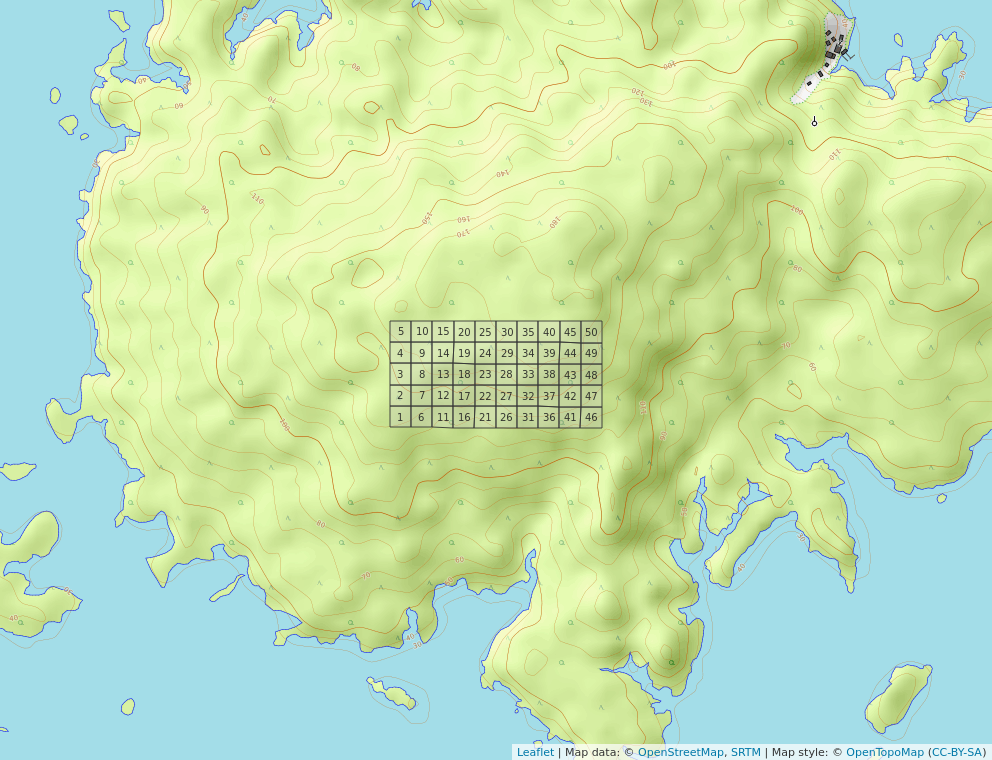
\includegraphics{mapa_cuadros.png}
\caption{\label{fig:mapa_cuadros}Organizacion de la parcela por
cuadricula de una hectarea}
\end{figure}

Con relación a la interpretación de las matrices, se tomó en cuenta la
distancia entre los sitios, dígase la disimilaridad (a mayor distancia,
mayor disimilaridad), la cual se representa usando la métrica de la
distancia euclídea, lo que equivale a una matriz de comunidad
transformada, en este caso a una matriz de Hellinger, ésta se
representará de forma gráfica en un mapa de calor con diversos colores,
el 1er mapa no representa ningún orden, mientras que el 2do sí,
facilitando así determinar patrones o grados de asociación.

\ldots

\section{Resultados}\label{resultados}

La familia Euphorbiaceae estuvo representada por 10 especies y un total
de 2421 individuos. La más rara, es decir, la menos abundante, fue
\emph{Alchornea latifolia}, con un solo individuo, seguida de
\emph{Sapium broadleaf} con dos individuos. La más abundante fue
\emph{Acalypha diversifolia}, con 1023 individuos (ver tabla
\ref{tab:tabla_de_abundancia} y figura \ref{fig:abun_sp_q}). La
distribución de la riqueza y la abundancia por sitios es desigual, con 6
especies y ca. 50 individuos en promedio por cuadros de 1 Ha. Los
valores mínimo y máximo de riqueza y abundancia por sitios muestran que
se trata de una familia con mucha variabilidad en la parcela; en los
cuadros 10, 17 y 43 se registraron tan sólo tres especies, mientras que
en los cuadros 29 y 37 se registraron 8. Asimismo, la abundancia por
cuadros fue muy variable, registrándose en el cuadro 2 el valor de
abundancia mínima de 7 de individuos y un máximo de 162 individuos en el
cuadro 50.

\begin{longtable}[]{@{}lr@{}}
\caption{\label{tab:tabla_de_abundancia}Abundancia por especie de la
familia Euphorbiaceae}\tabularnewline
\toprule
Latin & n\tabularnewline
\midrule
\endfirsthead
\toprule
Latin & n\tabularnewline
\midrule
\endhead
Acalypha diversifolia & 1023\tabularnewline
Croton billbergianus & 631\tabularnewline
Alchornea costaricensis & 316\tabularnewline
Adelia triloba & 143\tabularnewline
Hieronyma alchorneoides & 118\tabularnewline
Hura crepitans & 95\tabularnewline
Acalypha macrostachya & 52\tabularnewline
Sapium glandulosum & 40\tabularnewline
Sapium broadleaf & 2\tabularnewline
Alchornea latifolia & 1\tabularnewline
\bottomrule
\end{longtable}

\subsection{Riqueza y abundancia}\label{riqueza-y-abundancia}

La distribución de la abundancia de especies por cuadros de 1 Ha fue
inhomogénea (ver figura 2). Tanto las especies comunes (e.g.~Acalypha
diversifolia, Croton billgergianus) como las de abundancia intermedia
(e.g.~Sapium glandulosum, Acalypha macrostachya), se distribuyeron de
manera desigual a lo largo de la parcela. \emph{Acalypha diversifolia} ,
es la especie más abundante ya que registró un muchos individuos por
cuadros de esta especie seguido de \emph{Croton billbergianus}. Un dato
más que nos arroja esta tabla es que estas mismas especies pueden
coexistir ya que se les ve en algunas cuadrículas en las que ambas
coinciden con una alta cantidad de individuos, estas cuadrículas
corresponden a la 23 y a la 50, mismas que poseen la mayor riqueza
global de la parcela (ver figura \ref{fig:cuadro_riqueza_global})Todo
esto nos guia no solo a ver la riqueza por individuo sino que también
por familia.

\begin{figure}
\centering
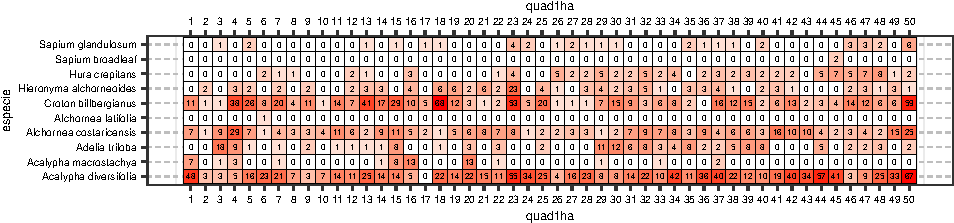
\includegraphics{manuscrito_files/figure-latex/unnamed-chunk-3-1.pdf}
\caption{\label{fig:abun_sp_q}Abundancia por especie por quadrat.La
gráfica representa la abundancia (celdas coloreadas en tonalidades de
rojo) de las especies de Eurphorbiaceae (ordenada) por cuadros de 1 Ha
de BCI (abscisa), a la izquierda esta la lista de especies y a mayor
intenso el color de la cuadricula, mayor es el numero de individuos}
\end{figure}

Las variables riqueza y abundancia de especies, tanto a nivel global
(todas las familias de plantas representadas en BCI) como respecto de
Euphorbiaceae, presentan un patrón espacial aglomerado, en algunos casos
insinuando el mismo patrón de distribución de determinadas variables
ambientales.

Concretamente, la riqueza de especies de BCI se hace máxima en las
celdas 23 y 50 (195 y 193 especies), con valores también altos en sus
vecinas. Respecto de la familia Euphorbiaceae, la riqueza de especies es
máxima en las celdas 29 y 37 (8 especies cada una), con valores también
altos en cuadros vecinos. En el análisis exploratorio no se detectó
correlación de la riqueza de especies de esta familia con ninguna de las
variables ambientales.

La abundancia sigue un patrón también aglomerado, pero distribuida de
diferente manera que la riqueza. Las celdas del borde noroccidental, con
valores que oscilan entre 4500 y 5000 individuos de especies de
distintas familias (ver figura \ref{fig:cuadro_riqueza_global}), forman
un aglomerado de la abundancia. Por otra parte, la abundancia de
especies de la familia Euphorbiaceae, mostró un patrón espacial similar
al de la riqueza de especies de BCI, siendo máxima en las celdas 23 y 50
(147 y 162 especies), con valores de abundancia también altos en sus
vecinas. Este grado de concordancia espacial entre la abundancia de
especies de Euphorbiaceae y la riqueza global de plantas de BCI, resultó
también respaldado por una correlación significativa (r=rho=0.55,
p\textless{}0.01). Adicionalmente, la abundancia de especies de esta
familia presentó relación directa con determinadas variables
ambientales, como el hierro, la pendiente media y la heterogeneidad
ambiental, y relación inversa con el porcentaje de morfología de valle
registrado en los cuadros. (ver figura \ref{fig:cuadro_riqueza_global}).

Esto abre una puerta a más variables determinantes que influyen el la
presencia, distribución y riqueza de las especies,esto se debe a que la
variación del relieve, tipo de vegetación, influye directamente el
clima, humedad, suelo, temperatura y muchos más factores que son
imprescindibles para la presencia de ciertas especies, esto aplica para
todo ser vivo, no de forma exclusiva a Euphorbiaceae. (ver figura
\ref{fig:cuadro_de_riqueza_familia})

\begin{figure}
\centering
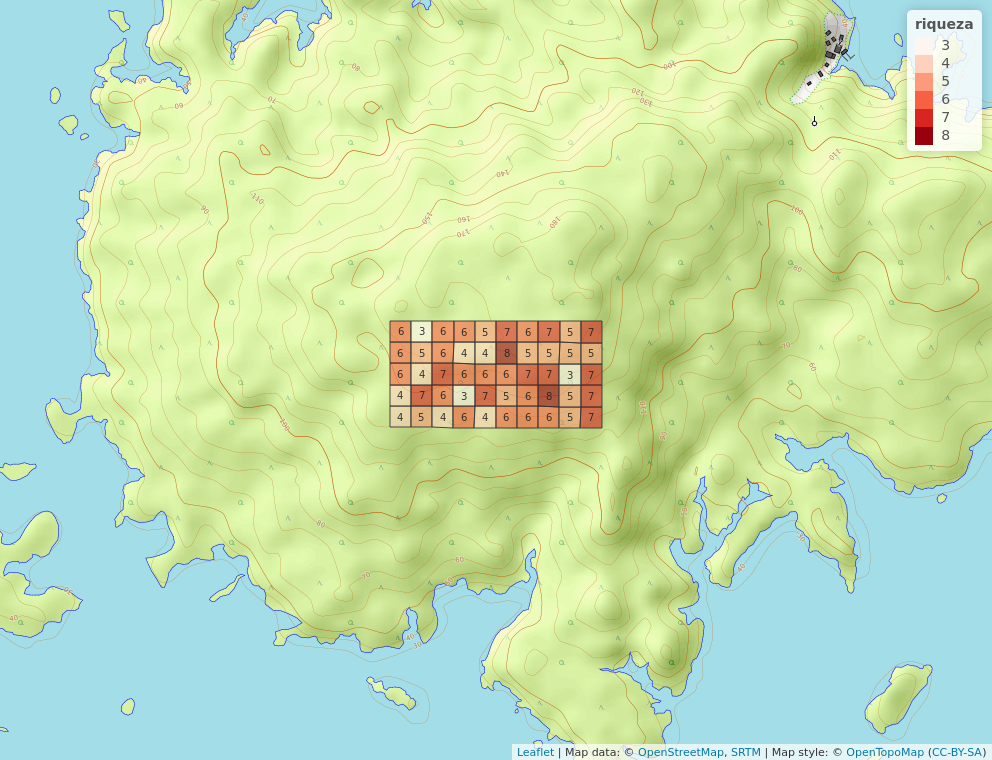
\includegraphics[width=0.50000\textwidth]{mapa_cuadros_riq_mi_familia.png}
\caption{\label{fig:cuadro_de_riqueza_familia}Representacion de la
riqueza de la familia Euphorbiaceae por cuadricula de una hectarea}
\end{figure}

\begin{figure}
\centering
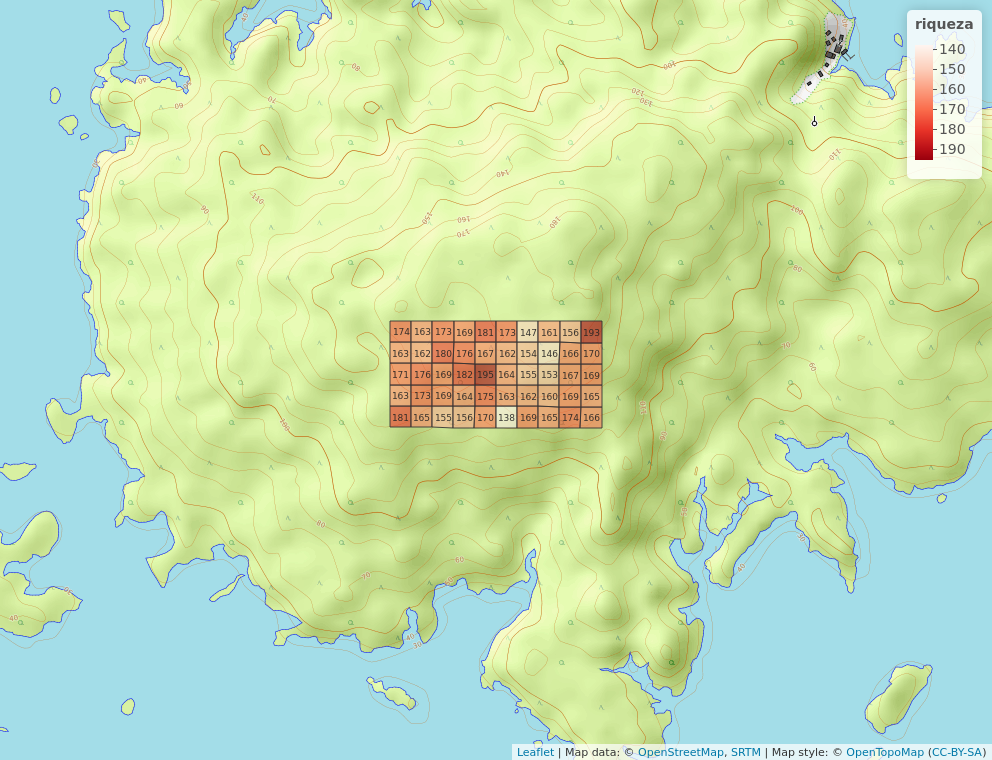
\includegraphics[width=0.50000\textwidth]{mapa_cuadros_riq_global.png}
\caption{\label{fig:cuadro_riqueza_global}Riqueza global}
\end{figure}

Comparando la abundancia global de nuestra familia de trabajo con la
abundancia global de especies podemos notar lo siguiente, existe una
asociación entre la abundancia global de especies y la abundancia global
de Euphorbiaceae y la inclinación, ya que las cuadrículas con mayor
cantidad de individuos también están situadas en la parte noroeste de la
parcela y la parte este también.(ver figura
\ref{fig:cuadro_de_abundancia_global})

\begin{figure}
\centering
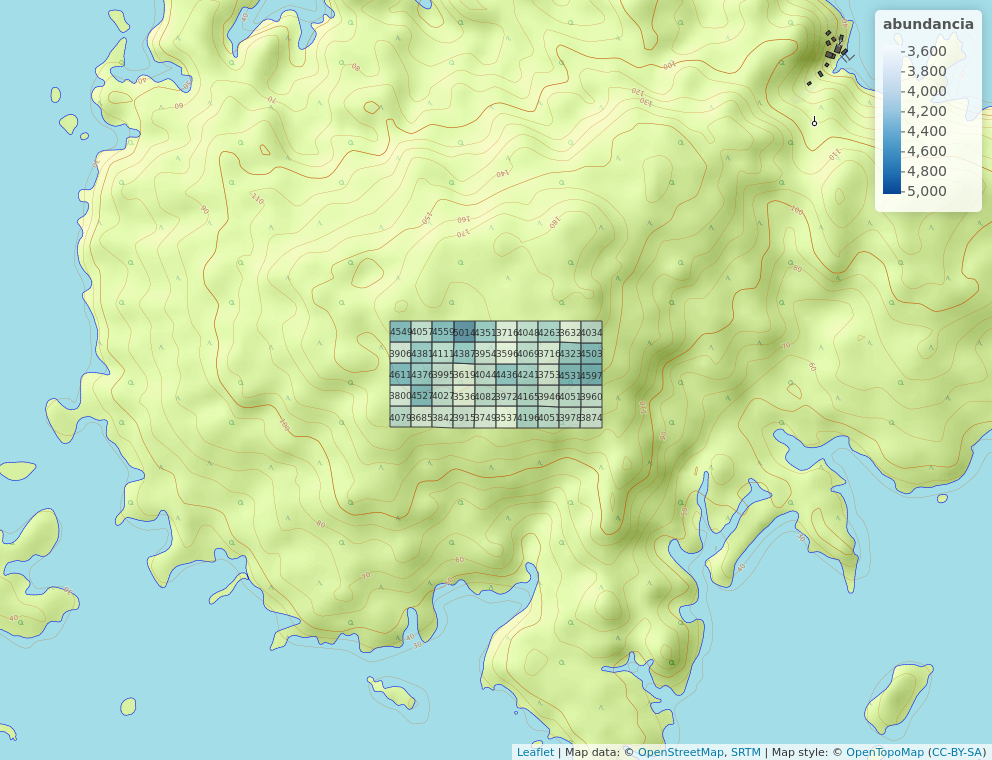
\includegraphics[width=0.90000\textwidth]{mapa_cuadros_abun_global.png}
\caption{\label{fig:cuadro_de_abundancia_global}Abundancia global}
\end{figure}

En cuanto a la abundancia de Euphorbiaceae, la cuadrícula 50 es la que
posee mayor cantidad de individuos seguido de la número 23 que se ubica
en la parte céntrica de la parcela con 147 individuos. En el mapa de
abundancia global se muestra el mismo patrón(ver figura
\ref{fig:cuadro_de_abundancia_global}),donde la cuadrícula 28 también
situada de forma céntrica, es una de las cuadrículas con más individuos,
4,436 para ser exactos, lo que me permite llegar a la conclusión que la
abundancia global de Euphorbiaceae está asociada a la inclinación del
relieve y la abundancia global de especies. Puede que haya un tercer
factor ( altitud, nutrientes, tipo de suelo,microclima,etc) que
determine la alta presencia de especies en esta zona y a la vez la alta
presencia de Euphorbiaceae.(ver figura
\ref{fig:cuadro_abundancia_de_mi_familia})

\begin{figure}
\centering
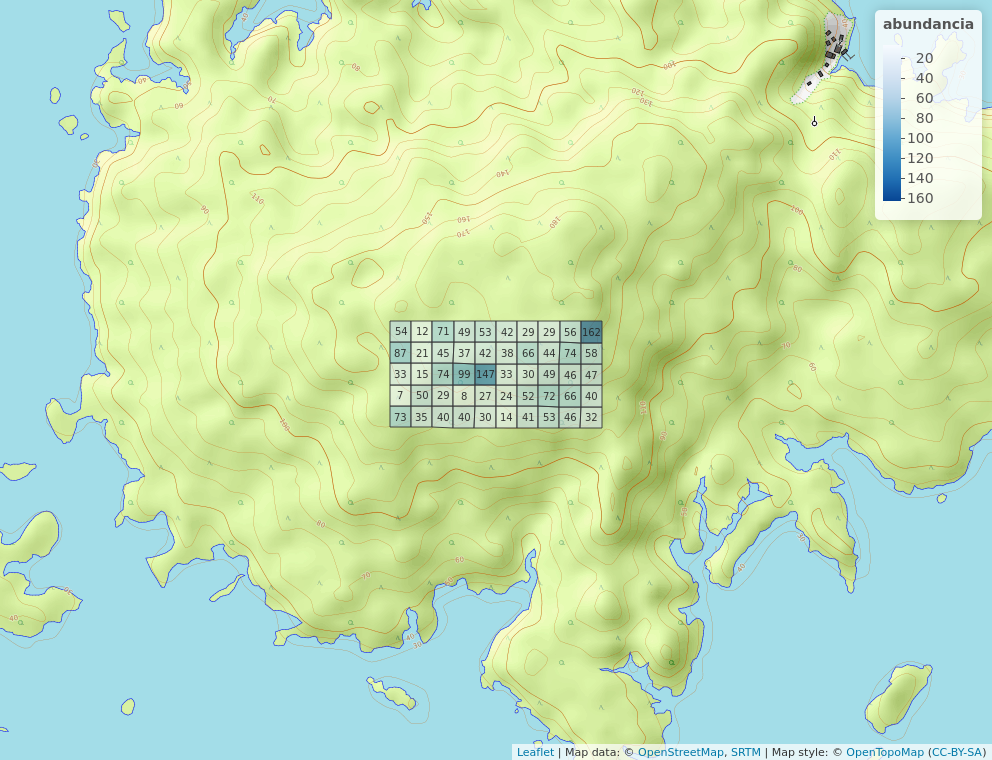
\includegraphics[width=0.85000\textwidth]{mapa_cuadros_abun_mi_familia.png}
\caption{\label{fig:cuadro_abundancia_de_mi_familia}Abundancia de
Euphorbiaceae}
\end{figure}

En el análisis de correlación de la riqueza y la abundancia de
Euphorbiaceae, sólo se detectó un patrón destacable: el contenido de
hierro del suelo presenta relación positiva y significativa con la
abundancia, no así con la riqueza. Son igualmente destacables, las
significativas asociaciones negativas y positivas que existen entre
distintas variables de suelo, aunque es común que múltiples variables de
suelo interactúen entre sí. (ver figura \ref{fig:suelo_ph_abun_riqu})

\begin{figure}
\centering
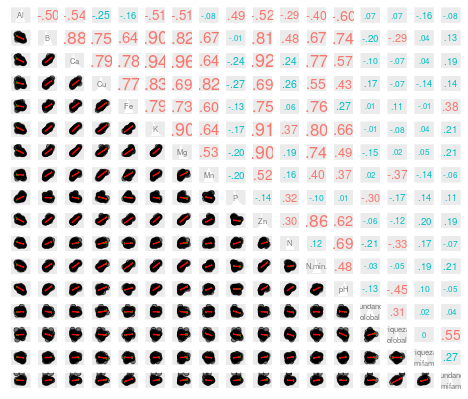
\includegraphics{suelo_ph_abun_riqu.png}
\caption{\label{fig:suelo_ph_abun_riqu}Relacion de elementos y ph del
suelo con la riqueza y abundancia de especies}
\end{figure}

Viendo la riqueza y abundancia desde una perspectiva de heterogeneidad
ambiental, según Pearson tomando en cuenta la geomorfología y los que
observamos es que hay variables como la elevación o la pendiente media
que muestran asociación con muchas de las variables del análisis, pero
los aspectos que nos interesan son relación entre la abundancia y
riqueza de Euphorbiaceae con las demás variables del análisis, y como
resultados tenemos que la abundancia de Euphorbiaceae muestra asociación
con la riqueza global de especies, al igual que con la pendiente media,
geomorfología del valle y la heterogeneidad ambiental, mientras que la
riqueza de nuestra familia solo muestra relación con con la
heterogeneidad ambiental y a diferencia de la abundancia no muestra
relación alguna con la riqueza global.(Ver figura \ref{fig:geo_pearson})

\begin{figure}
\centering
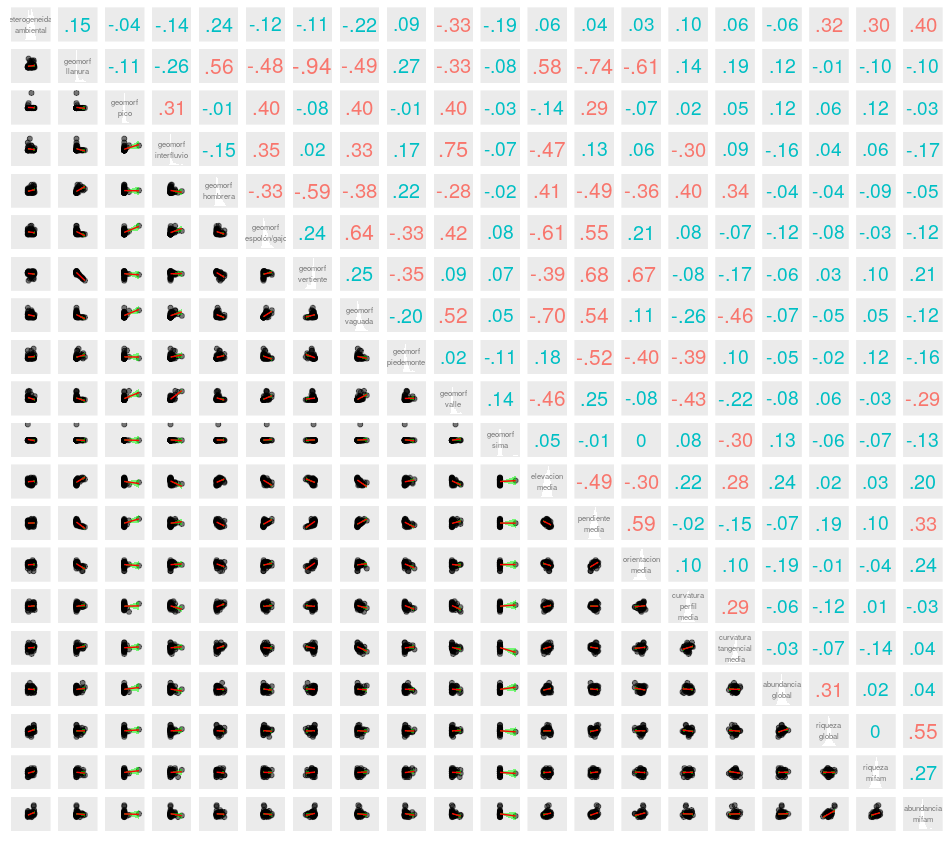
\includegraphics{geo_pearson.png}
\caption{\label{fig:geo_pearson} Relacion entre la Heterogenidad y
geomorfologia con respecto a la abundancia y riqueza de Euphorbiaceae
según Pearson}
\end{figure}

Pero desde la perspectiva de Spearman sólo la abundancia de nuestra
familia es la que muestra relación con las mismas variables que resaltó
el análisis de Pearson: riqueza global, geomorfología valle y
heterogeneidad ambiental aunque muchas de las variables geomorfológicas
muestran asociación entre sí.(ver figura \ref{fig:spearman})

\begin{figure}
\centering
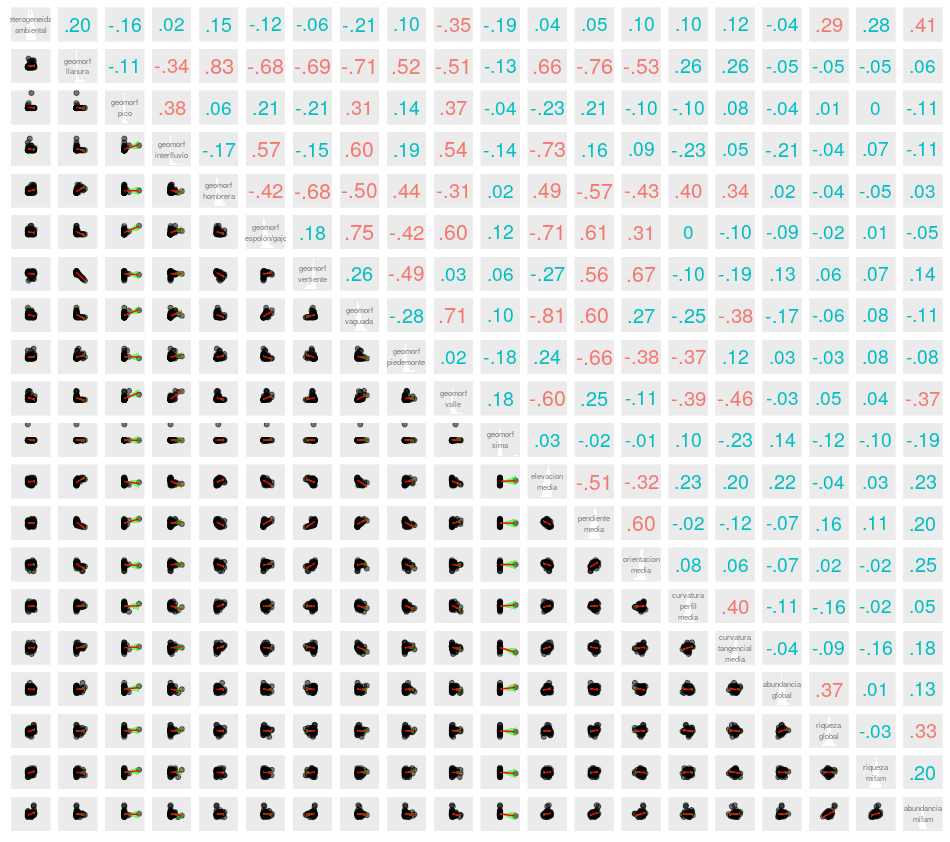
\includegraphics{spearman.png}
\caption{\label{fig:spearman}Relacion entre la Heterogenidad y
geomorfologia con respecto a la abundancia y riqueza de Euphorbiaceae
según Spearman}
\end{figure}

\subsection{MEDICIÓN ASOCIACIÓN}\label{mediciuxf3n-asociaciuxf3n}

El análisis estadístico de la asociación (relación, covarianza,
correlación) entre variables representa una parte básica del análisis de
datos en cuanto que muchas de las preguntas e hipótesis que se plantean
en los estudios que se llevan a cabo en la práctica implican analizar la
existencia de relación entre variables (Molina \& Rodrigo (2009)), que
es lo que veremos a continuación aplicado a nuestra familia.

La matriz de distancia euclídea calculada a partir de la matriz de
comunidad transformada por el método de Hellinger, revela que existen al
menos tres clusters claramente diferenciados. Un clúster grande
integrado por al menos 17 sitios (e.g.~sitios 25, 32, 33, 37, 50). Un
segundo cluster más pequeño de unos 4 sitios (e.g.~10,8,42,49) y un
tercer cluster compuesto por las cuadrículas 36,28,45,6, entre otras.
(ver figura \ref{fig:diss_hellinger})

\begin{figure}
\centering
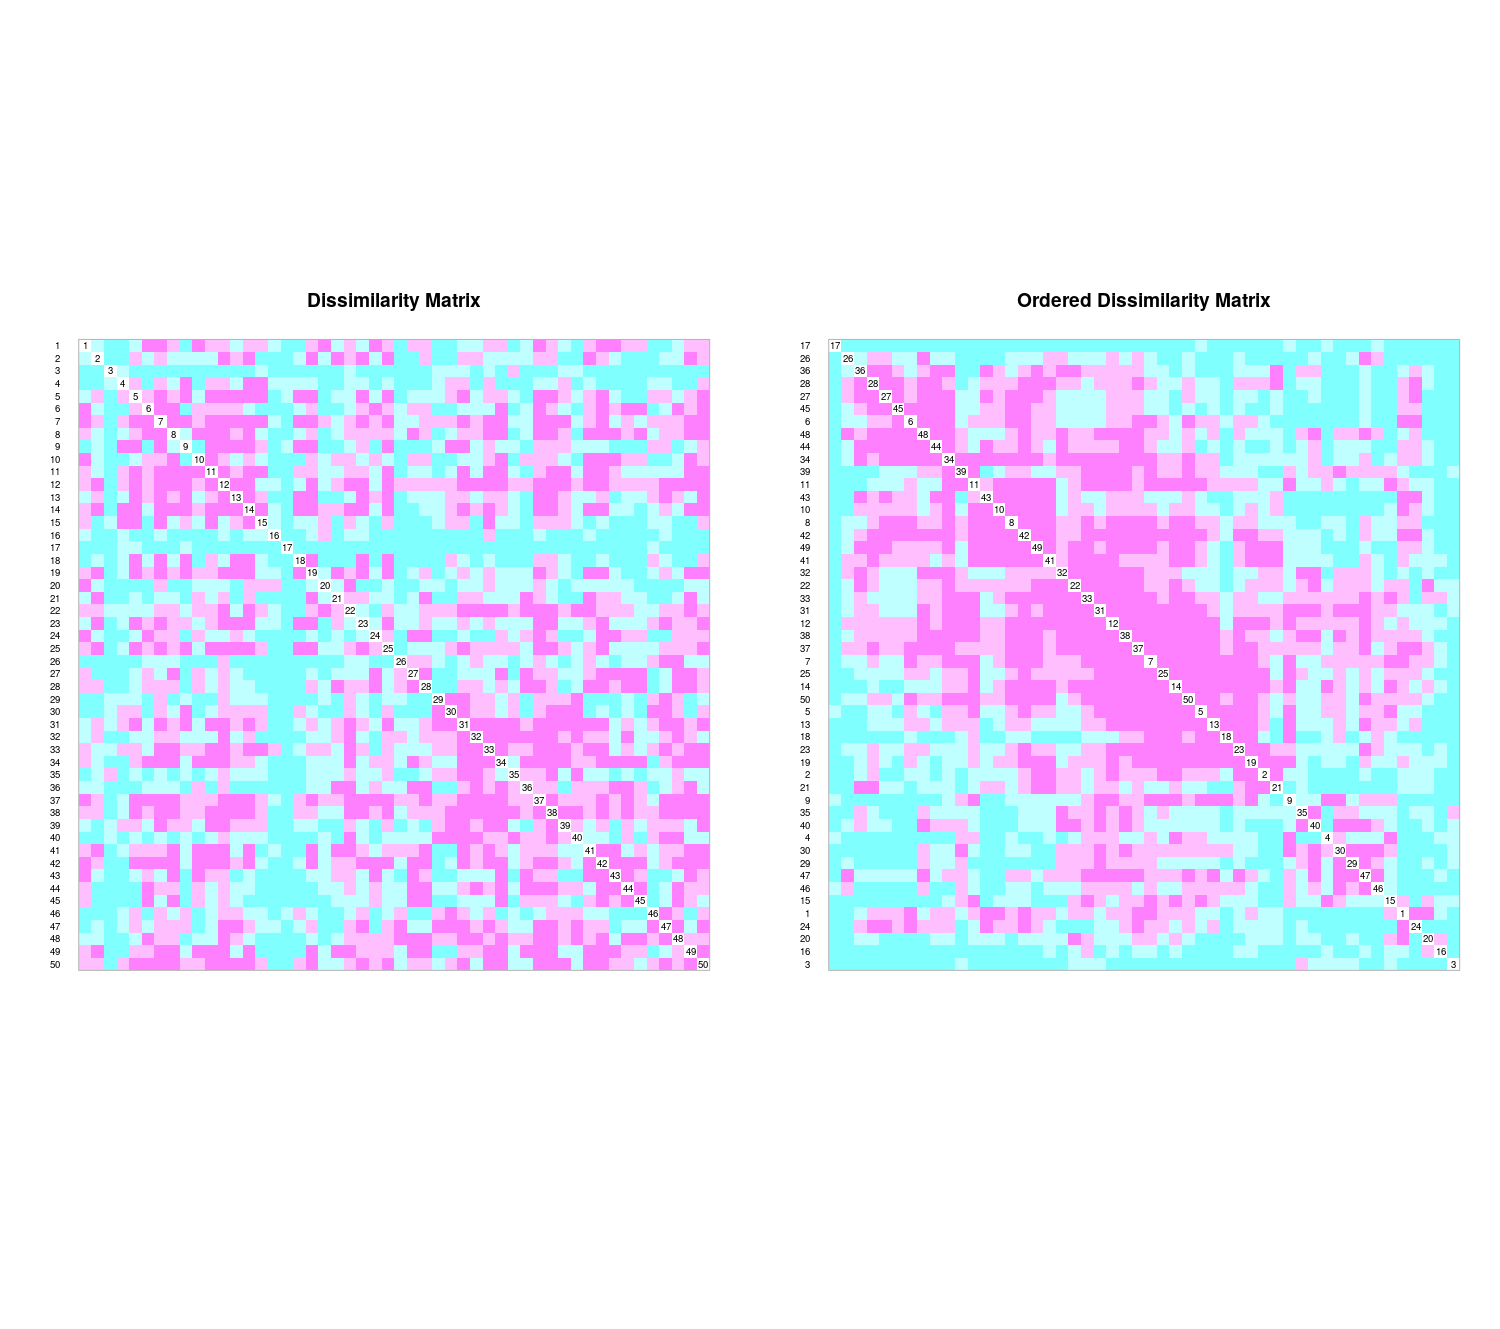
\includegraphics{diss_hellinger.png}
\caption{\label{fig:diss_hellinger}Matriz de Disimilaridad de
Hellinger,Rosa intenso: muy cerca, lila o rosa claro: distancia
intermedia; estan cerca, azul celeste o turquesa: larga distancia,
blanco: cero, un punto comparado consigo mismo}
\end{figure}

La zona de trabajo muestra un 91.7\% de similaridad o especies
compartidas, dándonos a entender que la riqueza de especies por
cuadrícula es bastante homogénea. Analizando la similaridad de Jaccard
para datos binarios (presencia/ausencia), lo que más resalta a primera
vista es un gran cluster formado por sitios digos un tanto aleatorio
(e.g.4,7,,18,20,29,30,35,37,38), y los sitios ubicados entre el 46 y el
50. Estos guardan especies compartidas haciéndolos sitios semejantes, en
otras palabras son sitios con poca disimilaridad en cuanto a sus
especies compartidas. Recordemos que a mayor distancia mayor
disimilaridad, lo que significa que desde el punto de vista de Jaccard
son muy parecidos y es interesante, ya que si observamos los números, no
todos los sitios de ese primer cluster están de forma continua en el
mapa y aun asi son similares. Algunos de estos puntos también coinciden
según Hellinger y puedes observar en la matriz anterior a esta, la
matriz de Hellinger siendo así importante el patrón entre las figuras de
las matrices 10 y 11. Si seguimos observando, hay clusters más pequeños,
los puntos 41,42,49,2,19 y 21 son parecidos entre sí teniendo poca
disimilaridad, también los sitios 1,43,10 y 24. (Ver figura
\ref{fig:diss_jaccard})

\begin{figure}
\centering
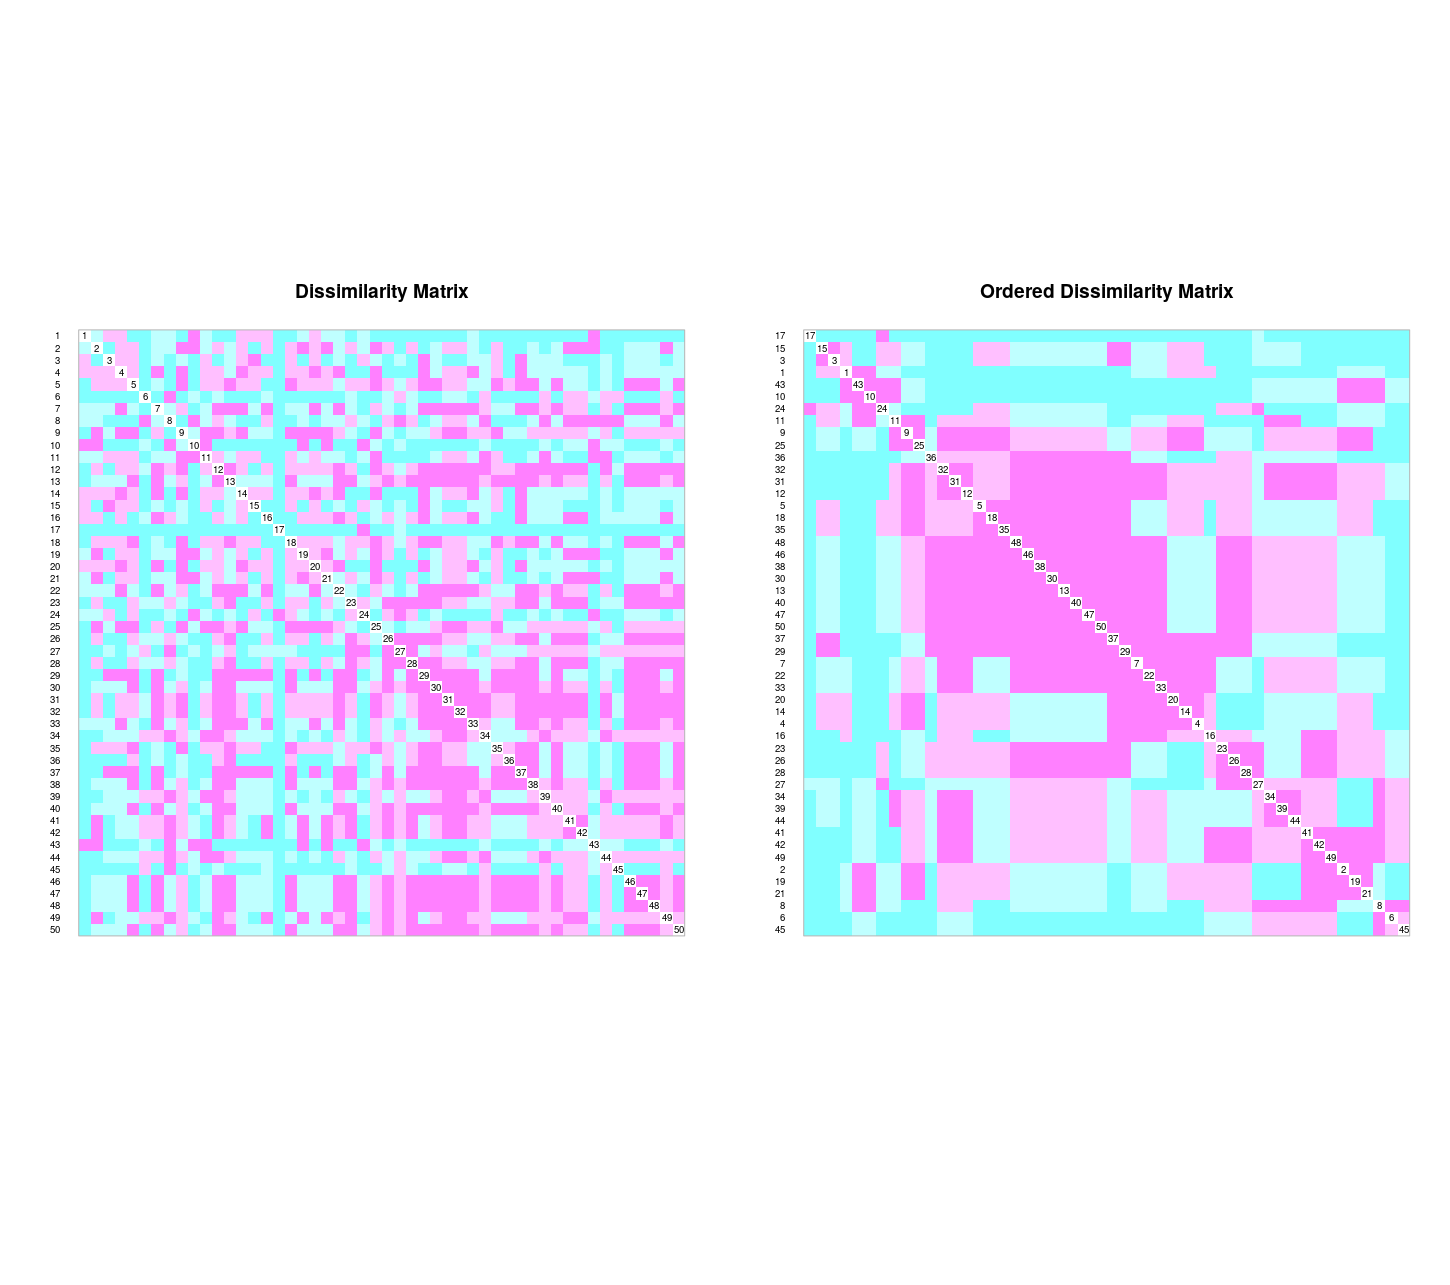
\includegraphics{diss_jaccard.png}
\caption{\label{fig:diss_jaccard}Matriz de disimilaridad de jaccard}
\end{figure}

Analizando la heterogeneidad ambiental basándonos en la topografía de la
zona, desde una matriz mixta, cuyas variables sean los tipos de
bosques(Old High;bosque viejo en relieve alto, Old Low;bosque en
vertiente baja, Old Slope;bosque relieve bajo, Swamp;bosque en área
encharcable y Young;bosque joven), el tipo de hábitat y
quebrada,presencia o ausencia de cañada (tabla de 3 columnas en nuestro
script de análisi), para determinar qué tan homogénea es la distribución
de los microhabitats en la parcela, podemos decir que los resultados
interpretados en base a la columna en el script y la matriz son: Los
niveles de heterogeneidad con respecto a microhábitat son bajos y pueden
ir desde 0.0000 a 0.6368, lo que nos dice que existe una gran
homogeneidad entre las microhábitat las hectáreas. Con relación al
hábitat, los más escasos son Swamp o bosque en área encharcable y Young
o bosque joven, en 1ro solo se encuentra en las cuadrículas 23 y 18 lo
que resulta razonable ya que ambas posiciones están contiguas de forma
longitudinal en la parcela, mientras que young o bosque joven está en
las cuadrículas 30 y 35 que al igual que la anterior, están de formas
continuas de forma longitudinal(el 23 a la derecha del 15), puedes
visitar la referencia 1 donde muestra la organización de la parcela por
hectárea y ubicar estos puntos para entender mejor.(Ver figura
\ref{fig:mapa_cuadros})

Las cuadrículas que coinciden con Old Slope son: cuadrícula
1,5,16,21,26,36,41,42,43,44,45,46 y 50. Las cuadrículas 1 y 5 están en
extremos opuestos, la 16 y 21 están contiguas de forma horizontal, lo
mismo pasa con la 26 y 36 aunque estas tienen la cuadrícula 31 de por
medio que posee un tipo de bosque diferente a estas, old low para ser
específicos, las 41,42,43,44,45 forman una una línea vertical con
respecto a la hectárea teniendo a las cuadrículas 46 y 50 en cada
extremo de esta línea, también resaltar que en las cuadrículas 1 y 50
hay presencia de quebrada. Tipo de bosque Old High está presente en las
cuadrículas 29,32,33,34,37,38,39 y 40, desde la 32 a la 34 están
posicionadas de forma vertical, esta última con la 29 a su derecha y
desde la 37 a la 40 también formas una línea vertical con respecto a la
parcela. Swamp (bosque en área encharcable) y Young (bosque joven)
fueron los dos tipos de bosques con menor frecuencia, el primero
presente en los sitios 23 y 10 y el segundo solo en los sitios 30 y 35.
EL tipo de bosque más abundante fue 0ld low, tipo de bosque en vertiente
bajo quebrada, presente en 26 de los 50 sitios y Swamp junto a Young
fueron los menos abundantes, cada uno presente en 2 sitios.

Debemos recordar que tanto la abundancia como la riqueza de nuestra
familia está asociada a la heterogeneidad ambiental según la correlación
de Pearson y que no hay tanto cambio brusco de tipo de bosque por sitio.
Esta matriz nos ayuda a entender el grado de diversidad \emph{beta} que
está presente en las cuadrículas, en este caso esta diversidad se
muestra muy homogénea para los Old slope, Old low y Young, ya que muchos
de los sitios con este tipo de bosque estas geográficamente contiguos,
donde no veríamos la diversidad \emph{beta} sería en Swamp ya que los
sitios con este tipo de bosque no están de forma continua como para
realizar comparación alguna al igual. (Ver figura \ref{fig:punt_z})

\begin{figure}
\centering
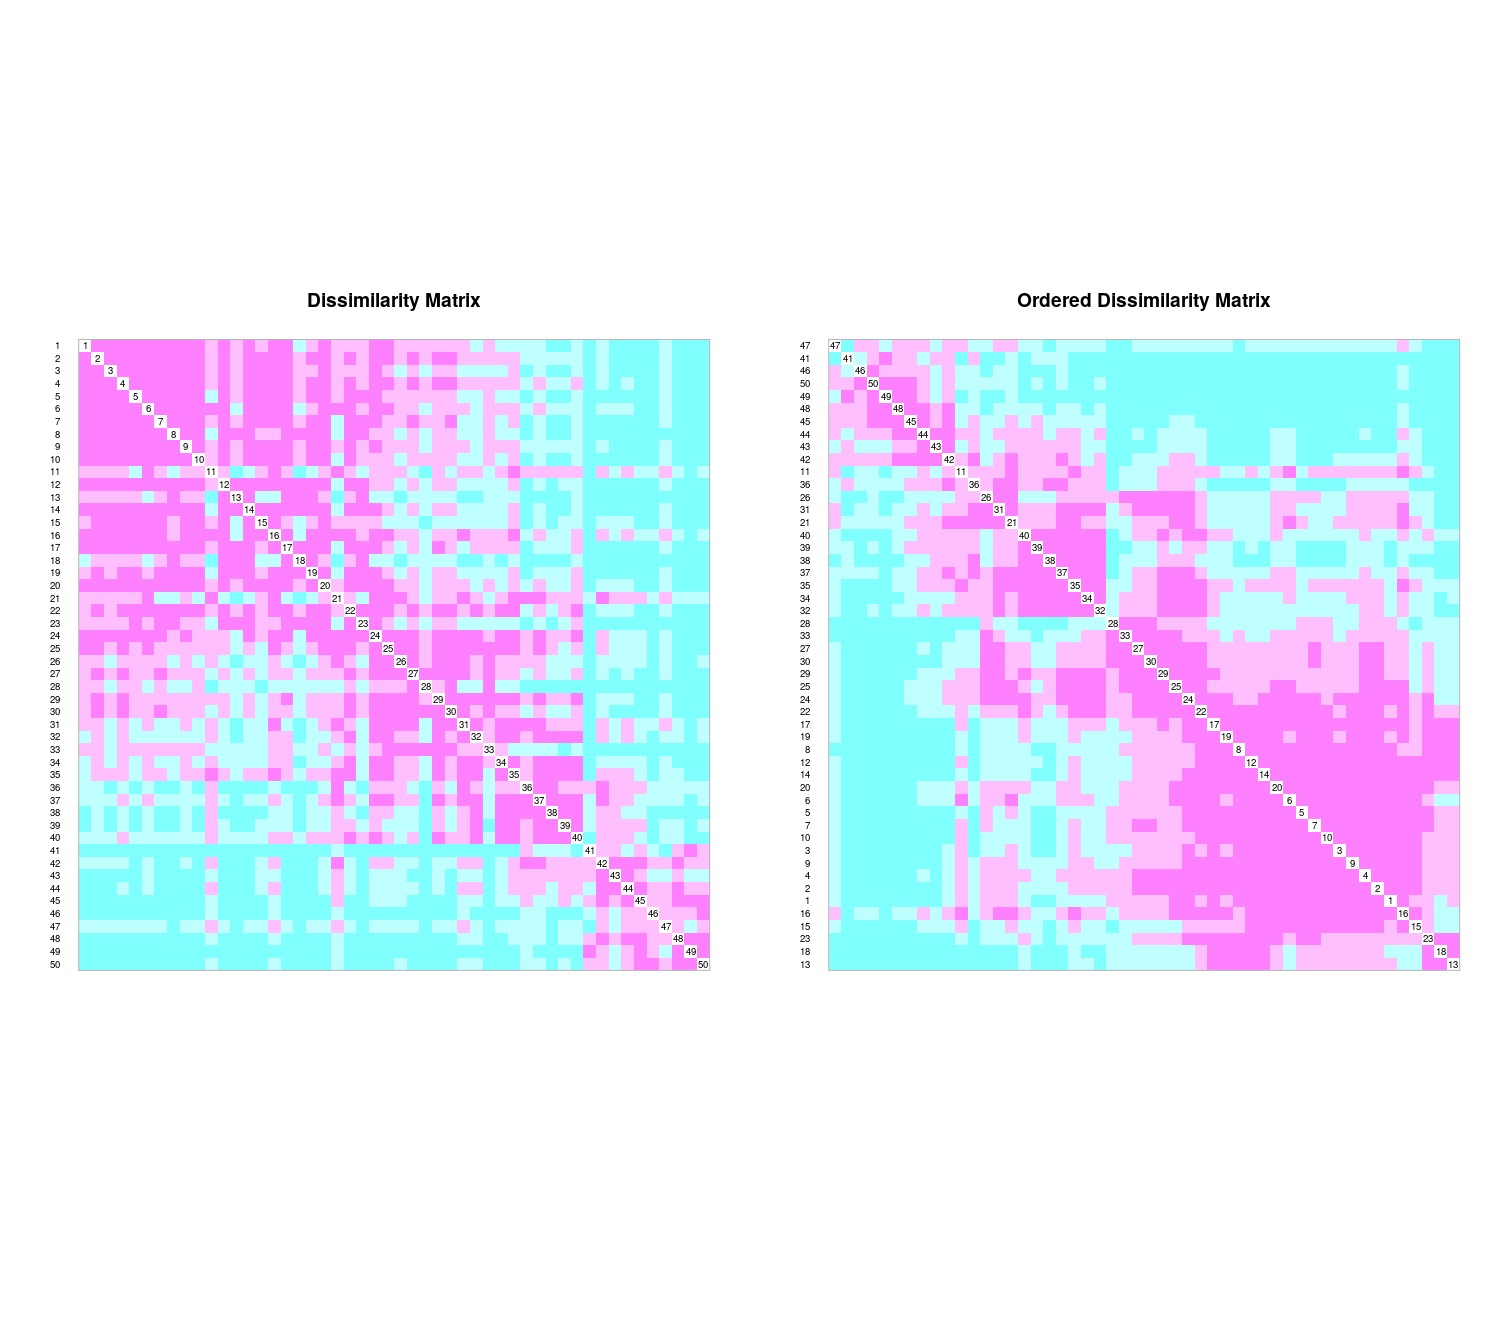
\includegraphics{punt_z.png}
\caption{\label{fig:punt_z}Matriz mixta}
\end{figure}

Al analizar la heterogenidad a través de una matriz transpuesta usando
datos de abundancia, para ver la posible asociación o patrones,tomando
en cuenta que estos datos también se analizaron mediante la
\emph{Correlacion de Pearson}, usando una matriz de comunidad en modo R,
donde dicha matriz se convirtió en datos binarios y los resultados
``brutos'' que arrojó mostraron consistencia, de los cuales obtuvimos
que: las especies relacionadas entre si están formando un único cluster
compuesto por \emph{Hieronyma alchomeoides}, \emph{Croton
billbergianus}, \emph{Acalypha diversifolia}, \emph{Hura crepitans},
\emph{Alchornea costaricensis} y \emph{Sapium glandulosum}. Algo
interesantes es que estas últimas dos mencionadas pertenecen al cluster
y pueden coexistir con las demás especies del cluster, pero no muestran
asociación la una de la otra. \emph{Acalypha macrostachya} solo muestra
una cierta relación con \emph{Alchornea costaricensis} siendo la que
menor distancia guarda entre especies no sitio y aún más leve con
\emph{Sapium broadleaf}, mientras que \emph{Alchornea latifolia} no
muestra asociación o cercanía con las demás especies, siendo así de las
que más distancia muestra con relación a las especies. Algo para
entender mejor este patrón, es si lo viéramos desde la perspectiva de
una correlación de nutrientes y variables de suelo. (Ver figura
\ref{fig:asoc_esp_no_sitio})

\begin{figure}
\centering
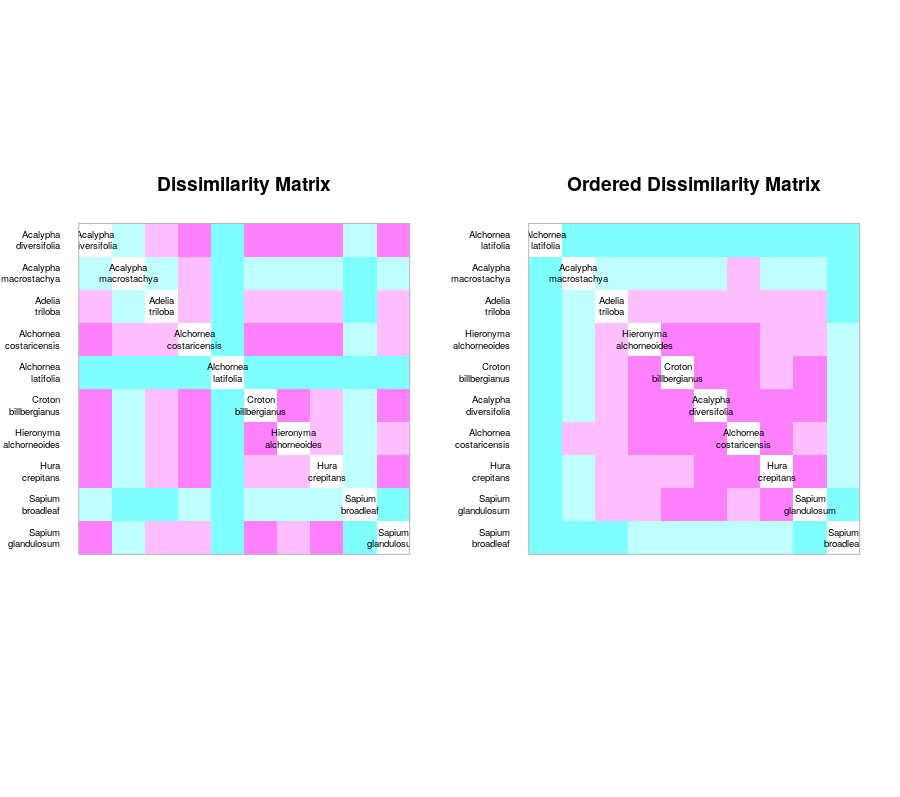
\includegraphics{asoc_esp_no_sitio.png}
\caption{\label{fig:asoc_esp_no_sitio} Matriz de disimilaridad entre
especies calculada a partir de una matriz de distancias ji-cuadrado,
donde se pueden explorar posibles patrones de co-abundancia}
\end{figure}

\subsection{Ordenación no
restringida}\label{ordenaciuxf3n-no-restringida}

Es importante ver si el ph y otros elementos del suelo se correlaciona
con nuestras especies, y esto podemos hacerlo a través de análisis de
PCA o análisis de componentes principales, CA o análisis de
correspondencia y PCoA o análisis de coordenadas principales, cada una
sus siglas en inglés.Estos nos servirán para ver el grado de asociación
que guardan los sitio y elementos del suelo. Debemos recordar que la
ordenación se basa también en la similaridad y que su principal
propósito es procurar reducir la dimensionalidad de los datos a través
de un conjunto de técnicas, como representar datos en ejes ortogonales
(comúnmente dos),donde el eje 1 explica la mayor varianza, el eje n
explica la mínima, etc.

Comencemos por PCA en un modelo de vara quebrada, pero antes aclarar que
la ordenación en este caso también se basa en la similaridad y que su
principal propósito es procurar reducir la dimensionalidad de los datos
a través de un conjunto de técnicas, como representar datos en ejes
ortogonales (comúnmente dos),donde el eje 1 explica la mayor varianza(la
mayor cantidad de varianza posible en el menor número de ejes), el eje n
explica la mínima, etc en este todas nuestras variables son numéricas y
comparables en cuanto a la escala de medición se refiere. los resultados
obtenidos a través de este análisis de componentes principales son los
siguientes: (ver figura \ref{fig:PCA_1})

\begin{figure}
\centering
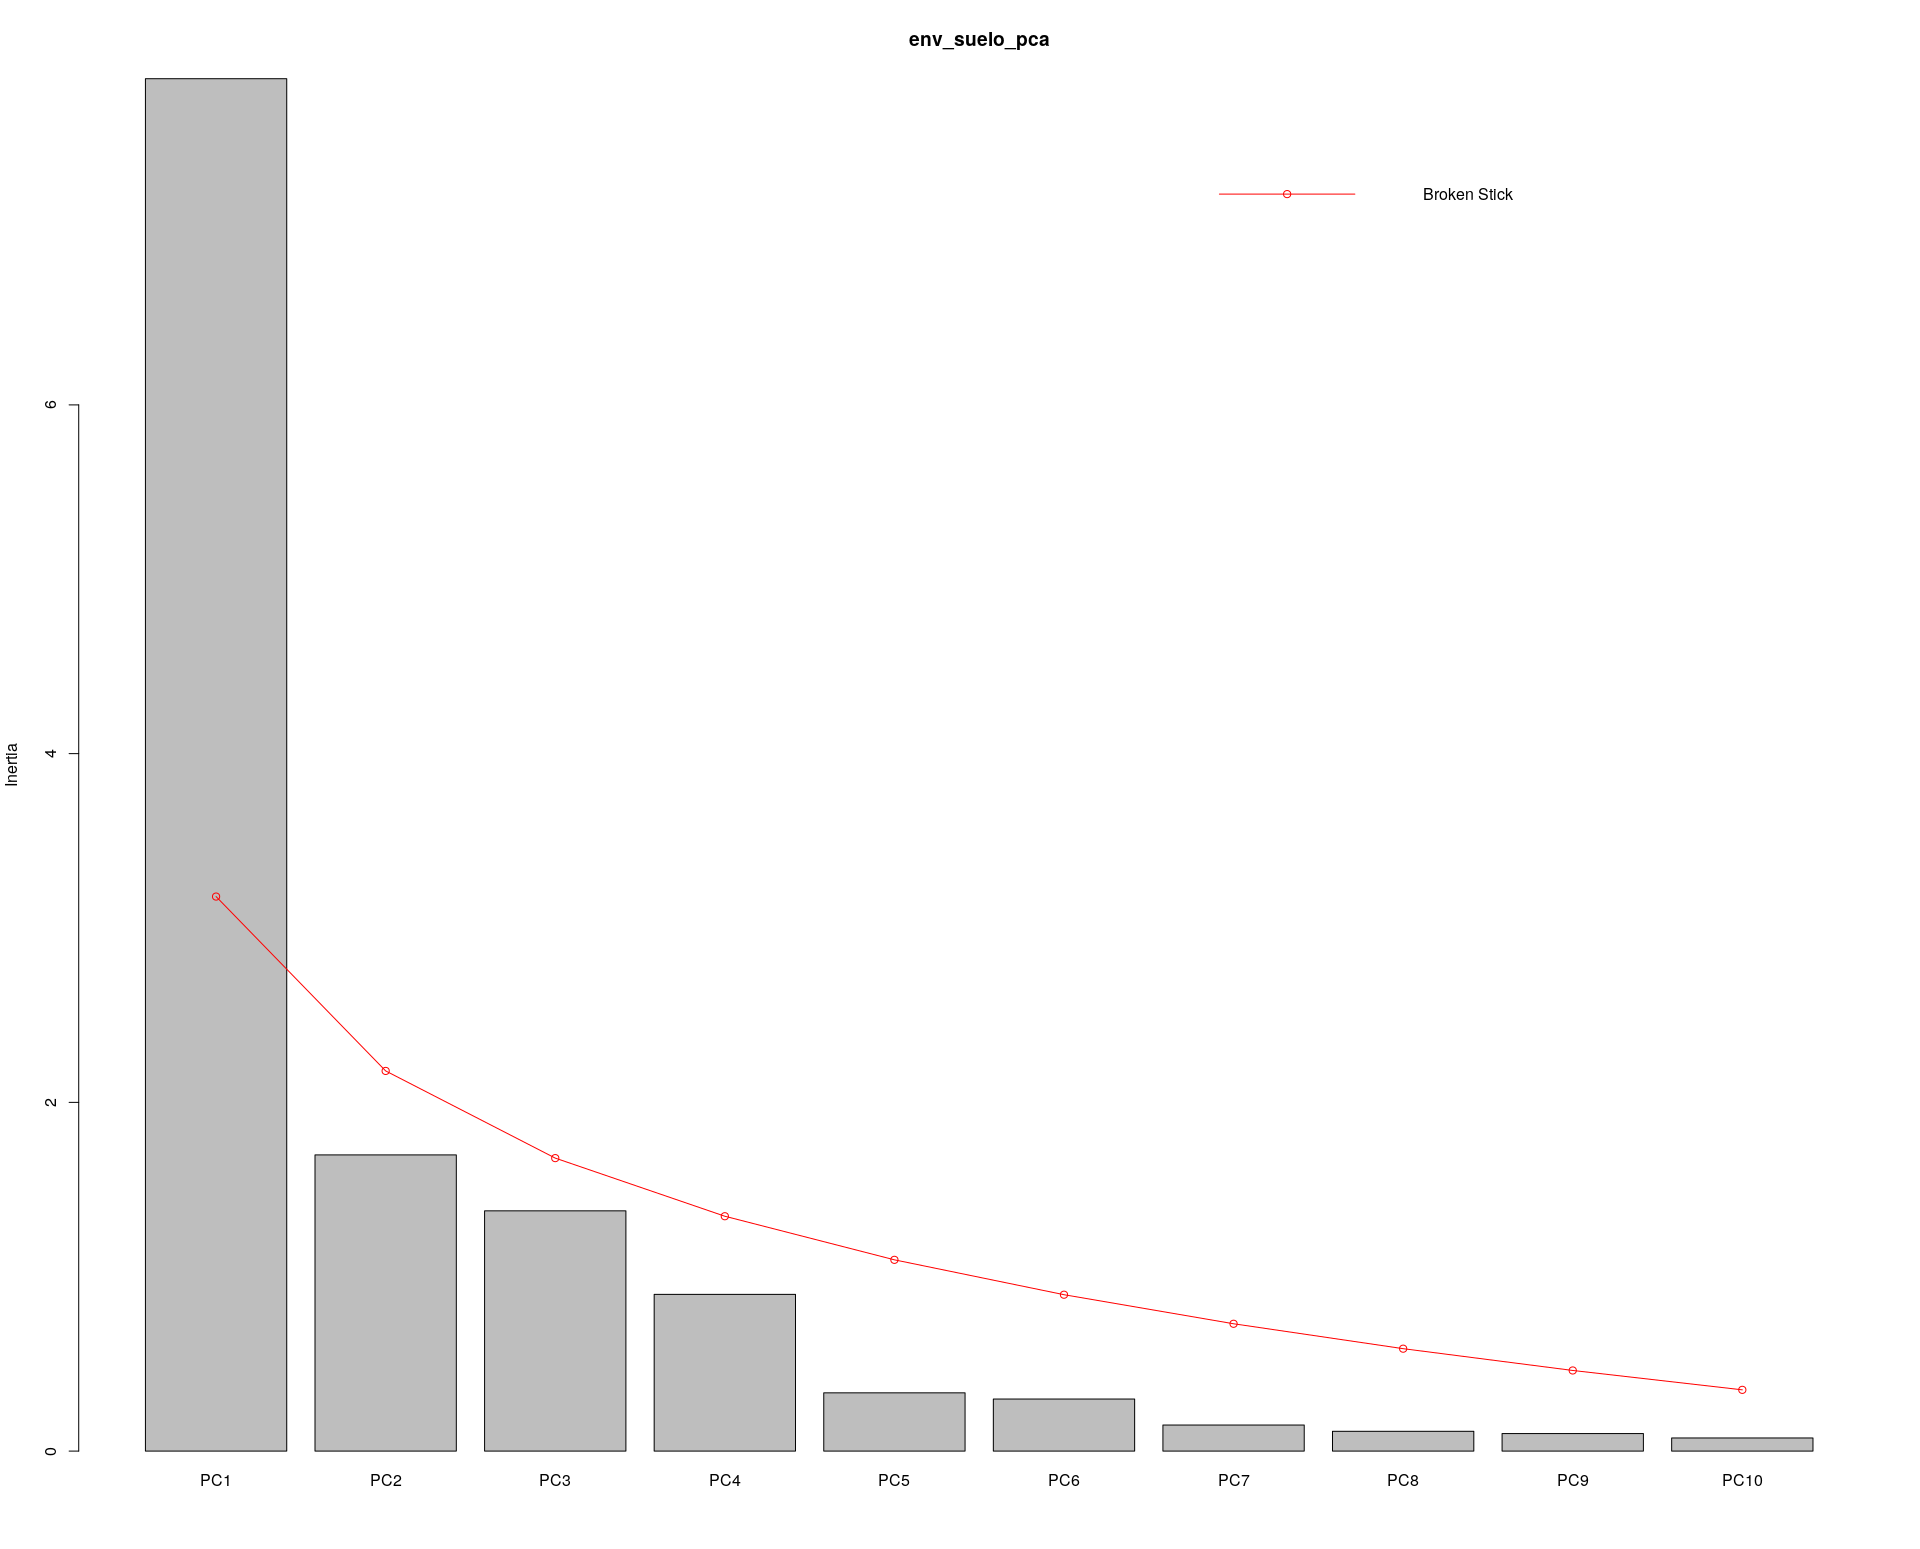
\includegraphics{PCA_1.png}
\caption{\label{fig:PCA_1}Presencia ausencia(Las barras representan los
valores propios de nuestros datos en cada una de las componentes y la
liena roja la vara quebrada)}
\end{figure}

Nuestro análisis de componente principal aplicado a la matriz de suelo
nos dice que el componente PC1 es importante y el resultado que nos
arroja es más de lo que se podría esperar para un modelo de vara
quebrada, un poco más que el doble, y que aporta suficiente varianza
para nuestra matriz, a diferencia de los demás componentes que no
sobrepasan la vara quebrada lo que nos indica que esos componentes son
pocos útiles ya que no consiguen explicar lo suficiente.

Viéndolo desde otra perspectiva, digase desde un Biplot, la correlación
se vería de esta forma: Podemos interpretar los datos de la siguiente
manera: la distancia euclídea está preservada en el escalamiento 1 y pH,
P y N son los componentes de suelo más abundantes en este escalamiento,
estos contribuyen mucho más en los componentes 1 y 2 y que en el resto
de los componentes,dígase poco equitativo, mientras que los demás
elementos o descriptores tiene una contribución para los demás los
componentes más o menos homogénea para cada uno de los sitios . En el
escalamiento 2 (distancia de Mahalanobis), el pH y el Nitrógeno guardan
una relación con los sitios 31,35,3637,38,39,40, mientras que ,
minerales como el hierro (Fe) y el aluminio (Al), están presente en casi
el 50\% de los sitios, siendos así muy parecidos en términos de
suelo(negativo). Otros puntos a resaltar son que los elementos Cu, Mn,
Fe están muy asociados, al igual que K y Zn, Ca,Mg Y N.min. lo que
significa que cuando uno crece el otro también, a diferencia de B y Al o
de P y Fe que cuando uno crece el otro disminuye porque no guardan
relación entre sí en otras palabras una relación inversa. (ver figura
\ref{fig:Biplot_pca1_pca2})

\begin{figure}
\centering
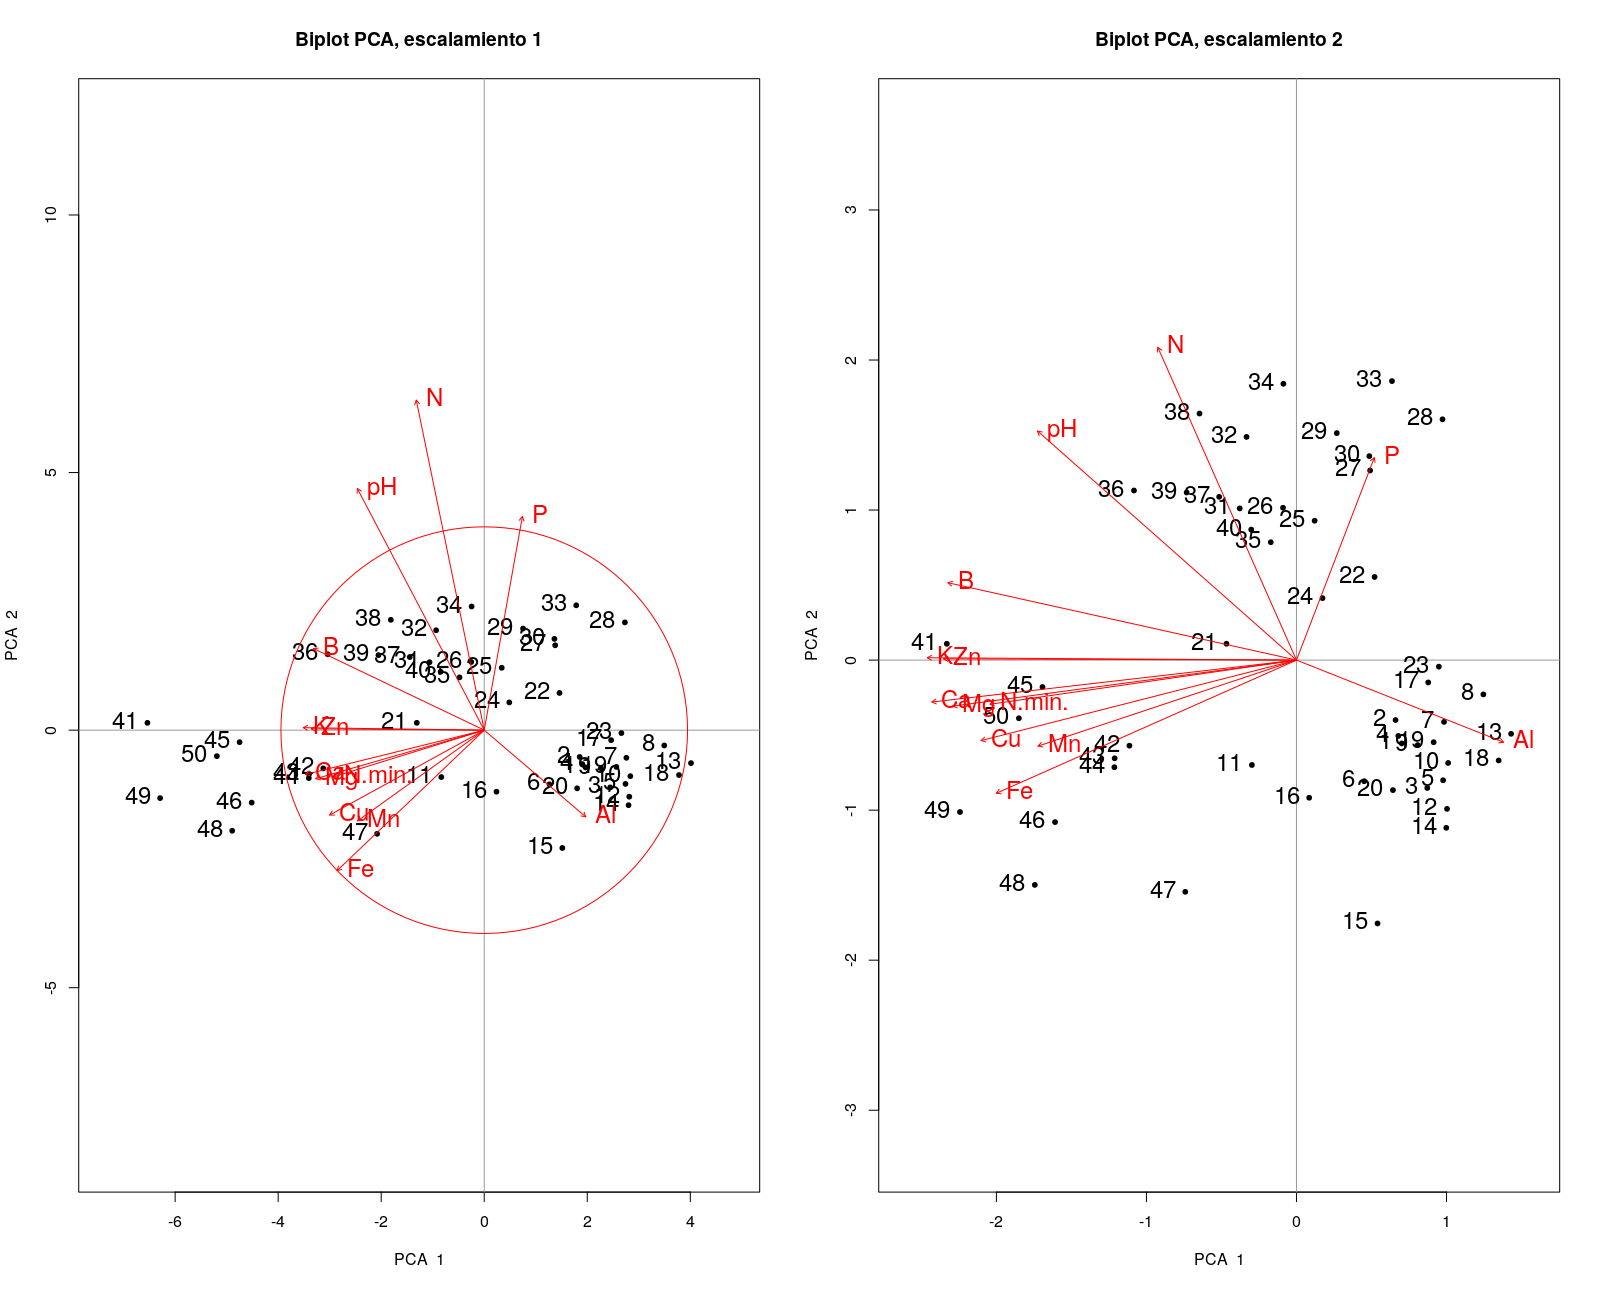
\includegraphics{Biplot_pca1_pca2.png}
\caption{\label{fig:Biplot_pca1_pca2}Recordae que el angulo entre los
vectores el lo que indica la correlacion estre ellos y que los sitiios
estan representados por puntos}
\end{figure}

Aunque las escalas son diferentes, podríamos decir que el patrón se
mantiene en ambos escalamientos ya que se presenta un agrupamiento de 3
cluster en ambos Biplot. aquí puedes ver un el conjunto de cluster en
función de los mismos datos de suelo, esta consistencia resulta
razonable aunque los métodos de ordenación no sean los mismos ya que
ambos se basan en la distancia euclídea. (ver figura
\ref{fig:cluster_pca})

\begin{figure}
\centering
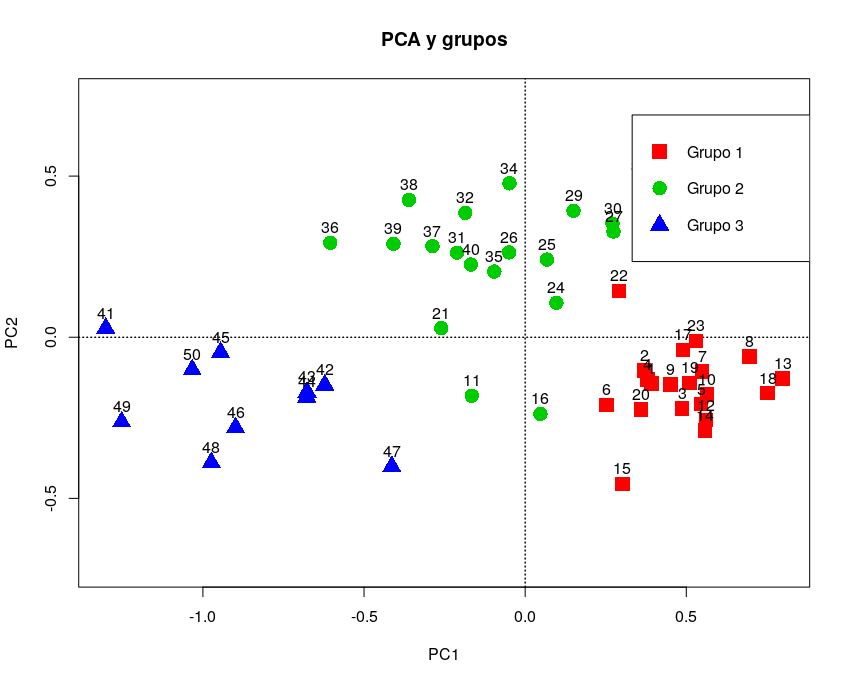
\includegraphics{cluster_pca.png}
\caption{\label{fig:cluster_pca}}
\end{figure}

Si aplicaramos en análisis de PCA para especies y no para variables
obtendremos ;lo siguiente: Nuestro modelo de vara quebrada quedaría de
la siguiente manera: el componente 1 a diferencia que el de datos de
suelo,este tiene poco más de lo que se podría esperar para el modelo de
vara quebrada, lo mismo pasa con el 2do componente pero en los demás no,
siendo estos dos primeros imprescindibles para el análisis de la matriz
de comunidad.Aun asi se podrian usar las primeras 4 o 5 componentes para
una mayor comprensión. (ver figura \ref{fig:quebrada_especie})

\begin{figure}
\centering
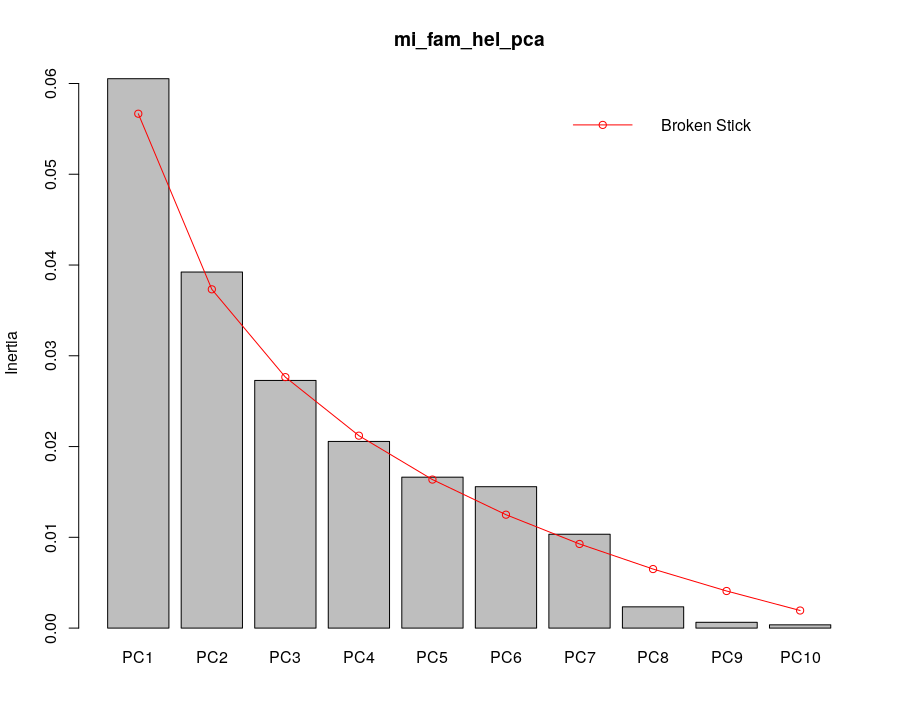
\includegraphics{quebrada_especie.png}
\caption{\label{fig:quebrada_especie}leyenda aqui}
\end{figure}

Viéndolo desde la perspectiva de diagrama de escalamiento o biplot,
obtendremos lo siguiente: (ver figura \ref{fig:biplot_especie})

\begin{figure}
\centering
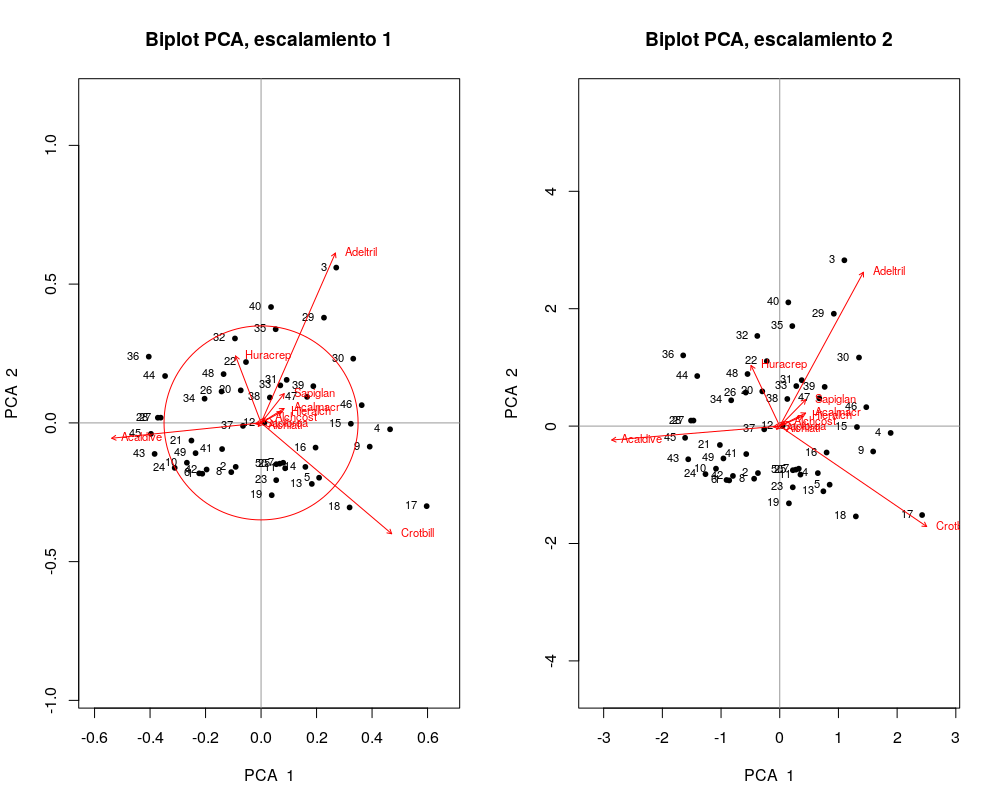
\includegraphics{biplot_especie.png}
\caption{\label{fig:biplot_especie}Resaltar que de este punto en
adelante, las especies están representadas por un acrónimo en cada
gráfico, cuyos equivalentes puedes encontrar en la información de
soporte del manuscrito.}
\end{figure}

Es de esperarse que los patrones no coincidan con el diagrama de
escalamiento anterior o biplot, y esto es porque las variables que se
están tomando en cuenta son diferentes. Anteriormente se usaban
elementos de suelo como descriptores y en este caso las especies de
nuestra familia Euphorbiaceae. Podemos ver que \emph{Acalypha
diversifolia} (Acaldive), junto a \emph{Croton billbergianis} (Crotbill)
y \emph{Adelia triloba} (Adeltil), son las especies menos equitativas en
los sitios de muestreo, cabe destacar que estas son más especialistas,
mientras que las especies cuyos vectores no sobresalen de la
circunferencia, con más generalistas.

Si correlacionar ambos análisis de PCA, tanto el de variables
ambientales y suelo con el de las especies obtenemos los siguiente: la
especie \emph{Croton billbergianis} posee una estrecha relación con el
aluminio, \emph{Hura crepitans} (Huracrep) con el Nitrógeno,
\emph{Acalypha diversifolis} también muestra cierta relación con el
potasio (K); los elementos pH, N, B, Y K poseen una estrecha relación
entre sí, especialmente el B y el pH. mientras que el K y el Al tienen
una relación inversa. (ver figura \ref{fig:suelo_especie})

\begin{figure}
\centering
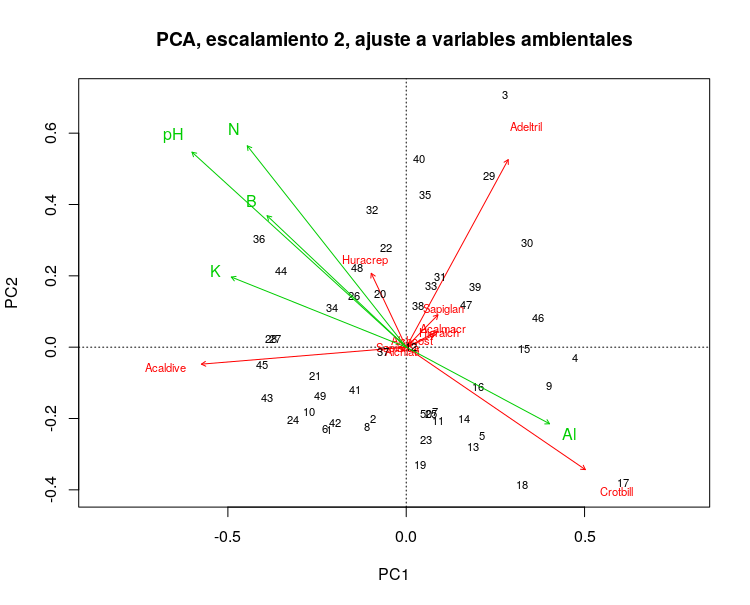
\includegraphics{suelo_especie.png}
\caption{\label{fig:suelo_especie}leyenda aqui}
\end{figure}

Si usamos solo las variables numéricas, obtendremos lo siguiente: N, Ph,
K, Al y B, siguen siendo variables significativas que pueden explicar la
distribución de especies, a las cuales se les suma Zn y Cu. También las
coordenadas UTM de este a oeste (UTM.EW) junto la riqueza global se
consideran variables significativas. En cuanto a la riqueza global, se
refiere al número de especie total por cuadro,la cual está asociado a la
matriz de comunidad como ya mencionamos, lo que significa que cuando
aumenta el número de especies, este puede ayudar a interpretar cómo se
distribuyen las especies dentro de la matriz de comunidad, dato que se
manifestó al principio en la correlación de Pearson.(Ver figura
\ref{fig:geo_pearson} Correlación de Pearson) (ver figura
\ref{fig:variables_numericas})

\begin{figure}
\centering
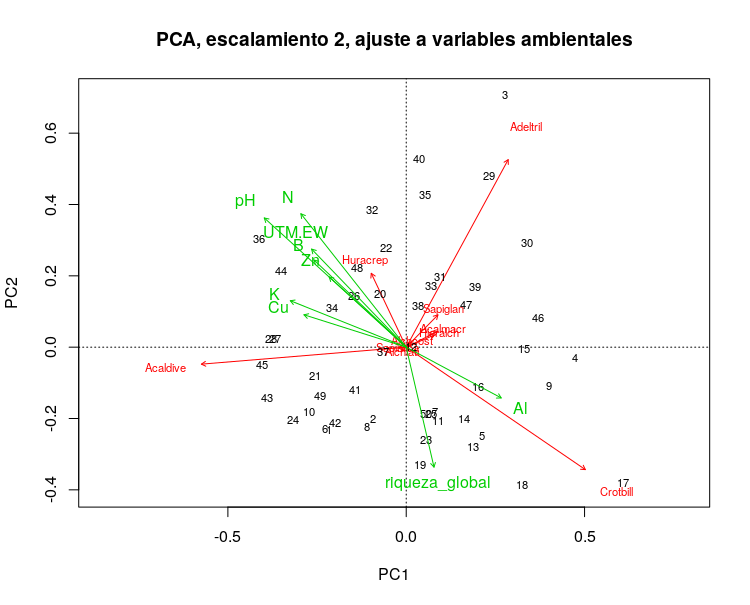
\includegraphics{variables_numericas.png}
\caption{\label{fig:variables_numericas}leyenda aqui}
\end{figure}

Una vez visto este análisis, pasemos al CA, análisis de correspondencia,
este es uno de los más usados y trata de llenar el vacío de las
limitaciones del PCA ya que este nos permite usar datos de conteos
aunque el CA no se puede aplicar a datos que no sean de frecuencias ya
sea de abundancia o de presencia ausencia y no es necesario transponer
las matrices. Está bien mencionar que en este análisis no trabajamos con
distancia Euclídea sino con la distancia ji-cuadrado.

Las distancias no van a coincidir del todo ya que se usan parámetros
diferentes pero de todas formas puede que resalten patrones ya vistos en
casos anteriores. El escalamiento 1 muestra la distancia en función de
sitios y el 2 la relación o distancia en función de especies.

Comencemos con el modelo de vara quebrada de nuestro CA, en este caso
los componentes CA2 y CA3, son los que podrían representar la matriz de
comunidad a diferencia de los demás modelos de vara quebrada donde el
componente 1 era el más explícito a nuestra matriz de comunidad.De todas
formas podemos usar las 4 primeras componentes para entender nuestra
matriz de comunidad y de esa forma entender y resumir el conjunto de las
multidimensiones de nuestra matriz de comunidad. Esto lo veremos mejor
explicado en los siguientes gráficos. (ver figura \ref{fig:AC})

\begin{figure}
\centering
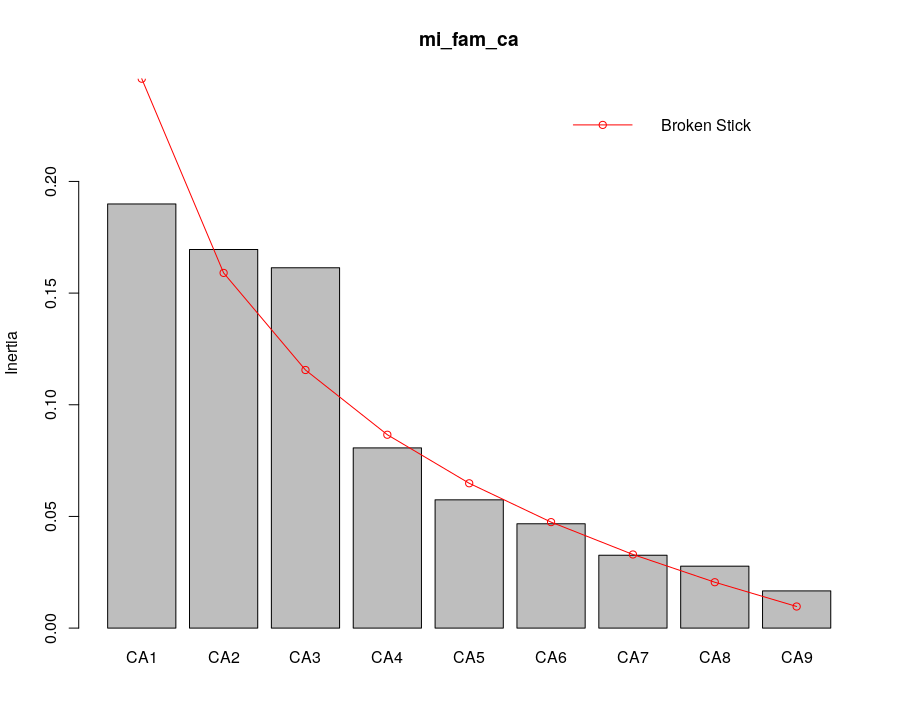
\includegraphics{AC.png}
\caption{\label{fig:AC}}
\end{figure}

Nuestros biplot del análisis de Correspondencia nos dicen lo siguiente:
no tenemos vectores, en este caso solo hay espacios comunes que muestran
la distribución y asociación. El biplot 1 o CA1 nos servirá para
entender la similitud entre sitios y viendo el gráfico nos dice que un
alto porcentaje de los sitios están más que relacionados,esto suele
pasar cuando nuestras especies no suelen ser tan especialistas, no
presentan patrones o tendencia muy clara. Hay unas 4 especies que rompen
este patrón: \emph{Adelia triloba}, \emph{Alchornea latifolia},
\emph{Acalypha macrostachya} y \emph{Sapium broadleaf}, en especial las
dos últimas, dándonos a entender que son especies algo más especialistas
y de poca abundancia, esto podemos evidenciarlo en la tabla de de
abundancia de especie por cuadrícula. (ver figura \ref{fig:abun_sp_q})

El biplot 2 nos servirá para ver la distancia entre especies, obtuvimos
lo siguiente: coincidiendo con el número 1, las especies guardan una
cercanía considerable, dando a entender que su patrón de distribución
podría ser homogéneo, aunque al igual que en el 1er biplot las especies
\emph{Adelia triloba}, \emph{Alchornea latifolia}, \emph{Acalypha
macrostachya} y \emph{Sapium broadleaf}, guardan una mayor distancia con
relación al resto, en especial las dos últimas, evidenciandola
consistencia entre los análisis.Las demás especies, por motivo de la
estrecha distancia ji-cuadrado, nos indica que están correlacionadas
entre sí.

En ambos biplots, \emph{Croton billbergianus} guarda cierta distancia
con relación a sitios y a especies, más en el 1er biplot que en el 2do,
pero no tanto como las especies antes mencionadas. (ver figura
\ref{fig:biplot_ca})

\begin{figure}
\centering
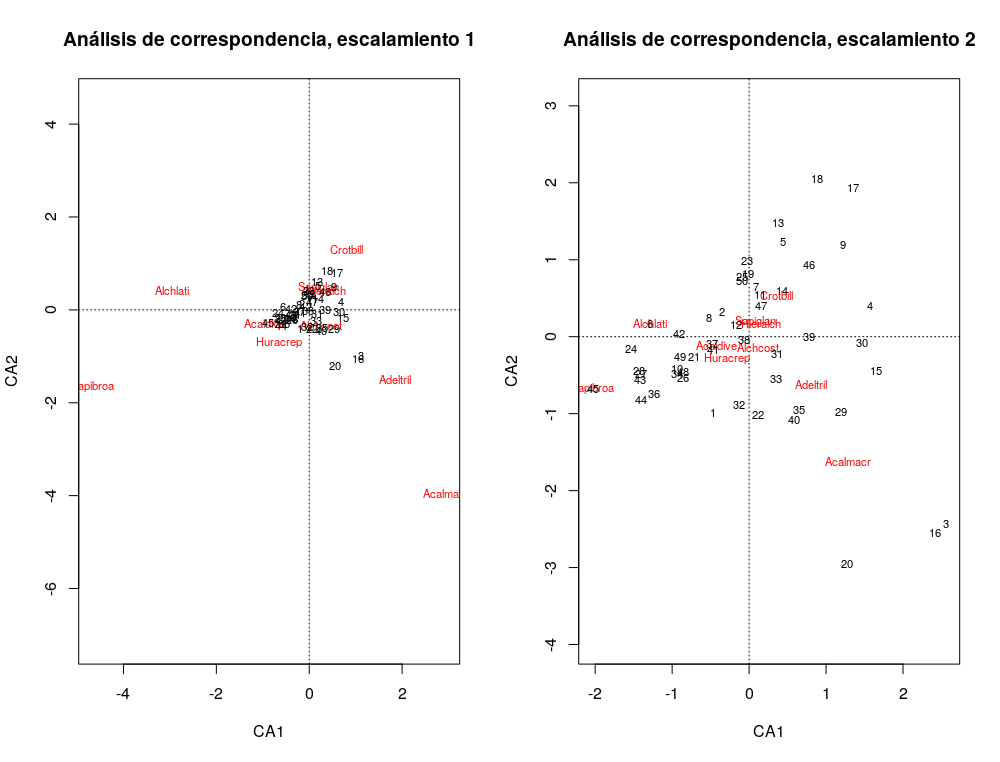
\includegraphics{biplot_ca.png}
\caption{\label{fig:biplot_ca}}
\end{figure}

Siguiendo con el PCoA o análisis de componentes principales en espa;ol,
este no usa la distancia euclídea ni la ji-cuadrada, lo que puede
resultar algo incómodo ya que esto nos resultara en vectores de
magnitudes negativas, imaginarias, dígase un vector complejo.Dicho
vector no se podrá aprovechar o representar como tal en el análisis de
coordenadas principales porque no se podrá representar en los ejes del
análisis.

Viendo los resultados de nuestro PCoA en el cual incluimos variables
ambientales y geomorfológicas, obtenemos lo siguiente: las especies que
muestran una contribución directa a sitios son, \emph{Sapium broadleaf}
que contribuye a los sitios 36,24,43 y 45, \emph{Alchornea latifolia} en
el sitio 48 y \emph{Adelia triloba} al sitio 19, aunque en la gráfica
las demás especies contribuyen no se muestran directamente asociadas a
un sitio en específico, estas contribuyen todos los sitios de manera
conjunta, también, las variables topográficas no muestras trascendencia
en este análisis a excepción de la heterogeneidad ambiental, riqueza
global y las coordenadas UTM de este a oeste (UTM.EW) que también se
hacen presente en los análisis anteriores.

Al igual que en los demás análisis, el Ph y el Nitrógeno (N) guardan
cierta relación pero en este caso muestran una relación aún más
estrecha. (ver figura \ref{fig:PCoA})

\begin{figure}
\centering
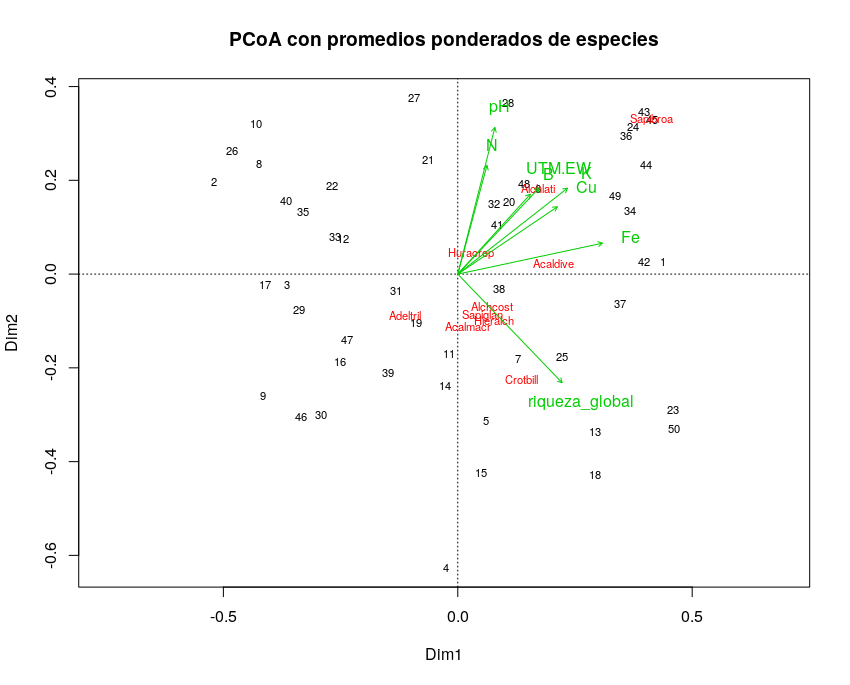
\includegraphics{PCoA.png}
\caption{\label{fig:PCoA}}
\end{figure}

\subsection{Ordenación restringida o
canóonica.}\label{ordenaciuxf3n-restringida-o-canuxf3onica.}

En estas también integraremos variables ambientales o de suelo, especies
y sitios, como variables explicativas, para determinar su integración,
pero estas no tendrán la misma libertad de moverse a como lo hacían en
la Teco no restringida ya que estos análisis posee restricciones por
ajuste por medio de regresión lineal con respecto a la matriz ambiental,
en otras palabras, buscaremos tendencias en una matriz de comunidad
restringida péndolas a una matriz ambiental. Esto lo haremos a través de
2 de los principales análisis de la técnica de ordenación no
restringida, estos serán: análisis de redundancia o RDA (siglas de
\emph{Redundancy Analysis}) Y análisis de correspondencia canónica o CCA
(\emph{canonical correspondence analysis}).

Comencemos por RDA que es el hermano canónico el PCA, este es una
combinación de una regresión lineal múltiple y el análisis de
componentes principales dando como resultado múltiples variables de
respuesta (multivariado). En este la exploración de datos es explícita
relacionada a dos matrices, una de respuesta y una explicativa, en donde
la matriz de respuesta equivale a la matriz de comunidad y la matriz
explicativa equivale a la variable ambiental.

Los resultados del RDA son los siguientes: En el escalamiento uno lo que
hace sentido es la distancia euclídea, por lo cual, lo resultante es un
cúmulo de los sitios de forma cercana. y en el escalamiento 2 los
ángulos entre especies y variables. El escalamiento 1 se vería de la
siguiente manera: A pesar de que los números están apiñados, podemos
diferenciar ciertos clusters, por ejemplo: los sitios 1,2,5,7,8,15
formas un pequeño cluster que muestra una asociación con el Al
(aluminio), al igual que el 13,14,19, otro pequeño cluster asociado al
Al y 46 y 47 muestran estrecha relación con P (fósforo), también las
especies como \emph{Hura crepitans}, \emph{Acalypha
diversifolia},\emph{Croton billbergianus}, entre otras, están muy bien
explicadas en este escalamiento y bien representadas en los sitios
contiguos al vector. (ver figura \ref{fig:RDA1_euclidea})

\begin{figure}
\centering
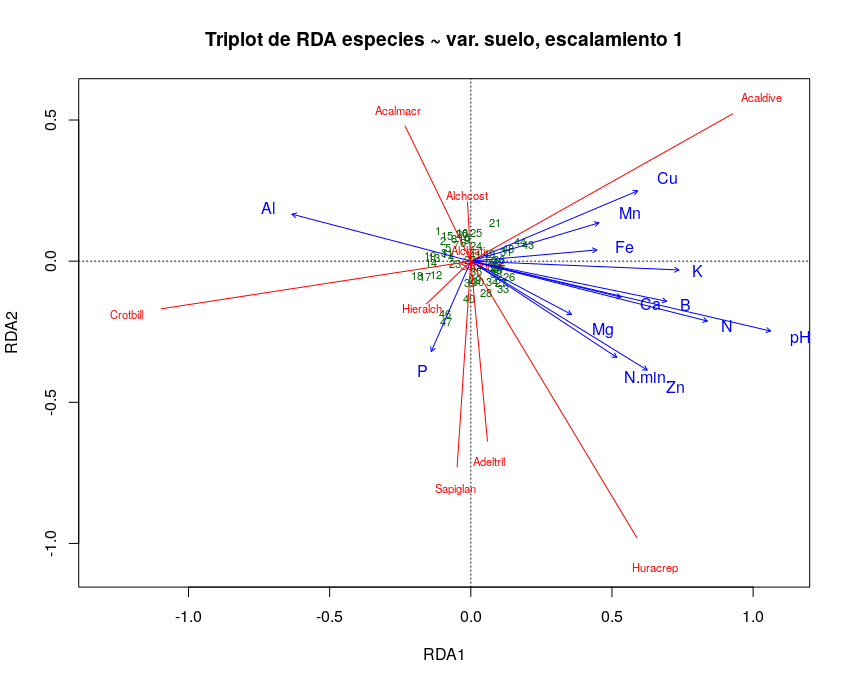
\includegraphics{RDA1_euclidea.png}
\caption{\label{fig:RDA1_euclidea}}
\end{figure}

Explicando la relación entre las variables explicativas en el
escalamiento 2, obtendremos lo siguiente: Las variables Ca,B,N y Ph,
muestran una estrecha relación entre sí, están presentes en los sitios
32,27 y 45 y que muestran una relación inversa con el aluminio
(Al).Tenemos un segundo cluster de Mg, Zn y N.min.(nitrógeno
mineralizado) con el Mg presente en el sitio 38, el Fe y K también
muestran cierta relación entre sí, en especial en los sitios 36,42,50,
el Mn y el Cu también están relacionados entre sí y presentes en los
sitios 31,43,44,48 y 49. (ver figura \ref{fig:RDA})

\begin{figure}
\centering
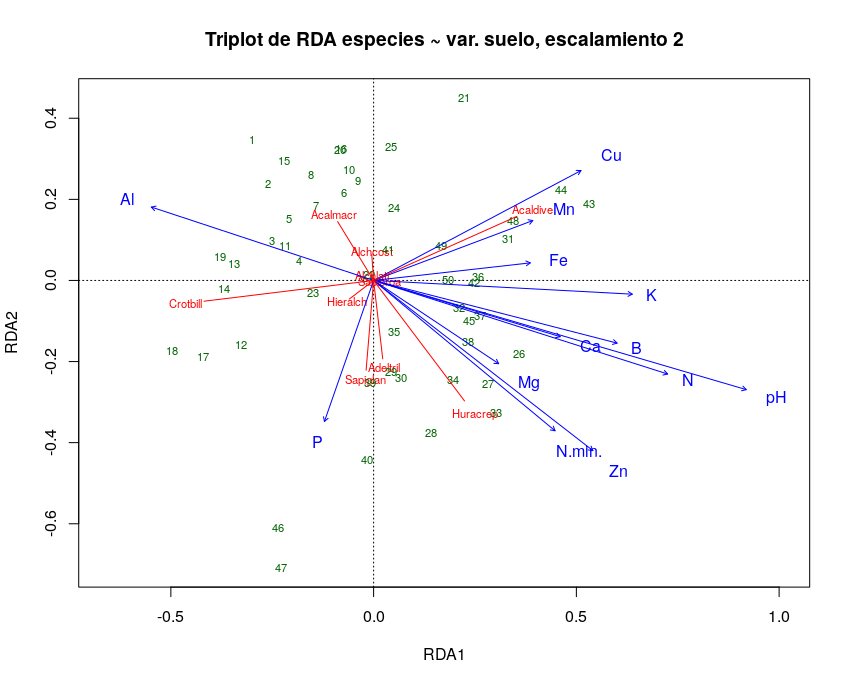
\includegraphics{RDA.png}
\caption{\label{fig:RDA}}
\end{figure}

También podemos añadir las variables que presentaron asociación en el
análisis pasivo de ordenación no restringida por PCA, y lo que vemos es
que aunque no existe colinealidad de forma directa, algunas variables
descriptivas forman ángulos bastante estrechos entre sí, indicando que
son variables muy relacionadas. Excluyendo variables asociadas al
análisis PCA de ordenación no restringida, basándonos en los valores VIF
que estas poseen, el resultado es que: de cierta forma, el Al y el N.min
poseen una relación inversa, las variables descriptivas B, N y Ph están
relacionadas entre sí de forma más directa en los sitios 36, 39 y 44,
mientras que el Cu no muestra asociación directa a las demás variables
explicativas pero si muestra contribución a sitios como el
24,25,34,38,41,42 y 43. (ver figura \ref{fig:PCA_RDA})

\begin{figure}
\centering
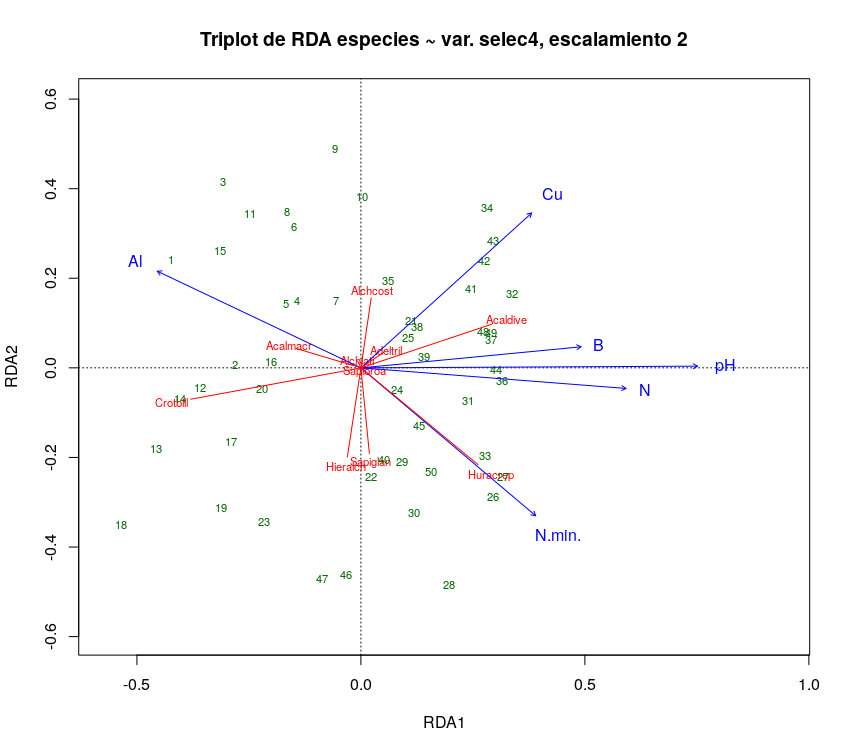
\includegraphics{PCA_RDA.png}
\caption{\label{fig:PCA_RDA}}
\end{figure}

Desde la perspectiva del nuestro segundo análisis de ordenación
restringida CCA, que es el hermano canónico del análisis de
correspondencia.en este análisis se realizó un ajuste a las variables
explicativas usando la distancia ji-cuadrado, de este tenemos los
siguientes resultados: en este caso la relación inversa del Al es con el
N y el Ph, elementos que guardan una estrecha relación entre sí,
formando un cluster junto al B. El N.min aporta de forma directa a las
especies \emph{Hura crepitans} (Huracreps) y \emph{Sapium
broadleaf}(Sapibroa) per no muestra estrecha relación con otras
variables explicativas, lo mismo pasa con el Cu pero este aporta de
forma más directa a \emph{Adelia triloba} (Adeltril), esta misma especie
junto a \emph{Acalypha diversifolia} (Acaldive) simulan ser especies
mineralizadas. (ver figura \ref{fig:CCA})

\begin{figure}
\centering
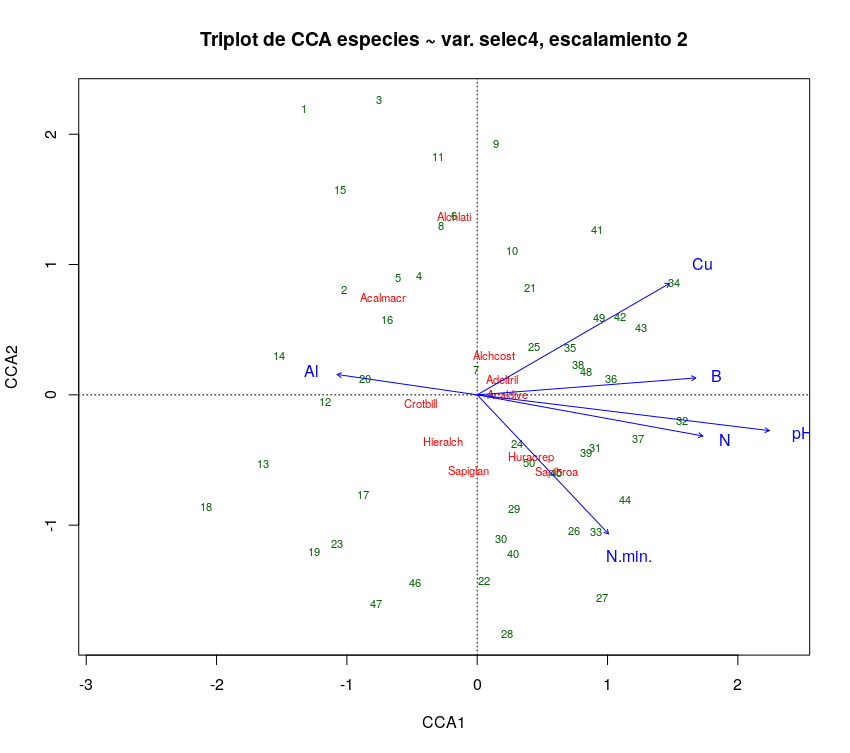
\includegraphics{CCA.png}
\caption{\label{fig:CCA}}
\end{figure}

Si mostráramos el mismo gráfico pero sin especies ``raras'', tomando en
cuenta que el concepto raro en este caso está aplicado a especies con
menos de 100 individuos, asi se explicaria mejor o estaria menos sesgado
los resultados con la distancia ji-cuadrado, tendríamos que nuestra
precisión pasaría de 0.1273683 a 0.1739327 y los resultados muestran que
en este caso la relación inversa del Al se muestra con el Cu y el
N.min.,\emph{Acalypha diversifolia} (Acaldive) sigue estando asociada al
Ph y de cierta forma aún guarda algún tipo de relación con el N y el B,
mostrando así un patrón de asociación con relación a estas variables
explicativas. Esto cambios brusco de la ordenación de las especies en
los diferentes análisis y sus respectivos gráficos, nos muestra la
variación de la diversidad \emph{alpha} con relación a las variables de
suelo, y demás variables descriptivas, dándonos a entender que dicha
diversidad no es homogénea para estos casos. (ver figura
\ref{fig:no_raras})

\begin{figure}
\centering
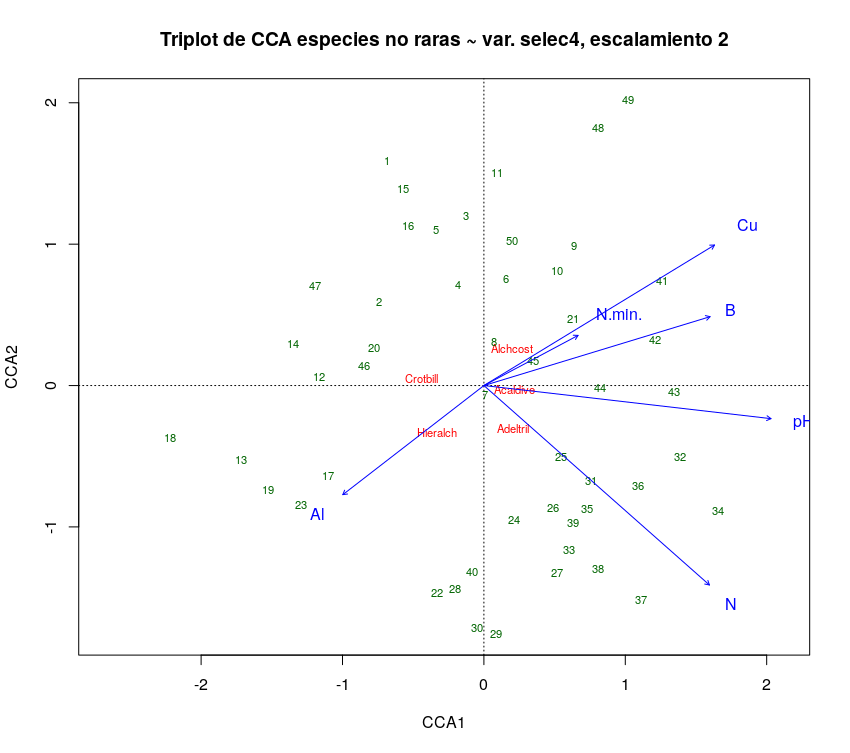
\includegraphics{no_raras.png}
\caption{\label{fig:no_raras}}
\end{figure}

\ldots

\section{Discusión}\label{discusiuxf3n}

A modo de discusión o más bien de conclusión, es evidente lo clara que
está la representación de la riqueza de Euphorbiaceae e incluso a que
variables descriptivas está asociada, información imprescindible para el
desarrollo de los análisis desarrollados. Los patrones de las especies
presentes en los diferentes tipos de bosque fueron de gran importancia
para entender cómo se manifiesta la diversidad beta en las cuadrículas
de la parcela y conocer las variables de suelo, contribuyeron a poder
ver a cuales están asociadas las especies y a predecir patrones de
abundancia basándonos en la presencia ausencias de estas variables.

Al procesar los datos de nuestra familia a través diversos análisis, nos
ayudaron a comprender la diversidad ecológica, la distribución,
abundancia y ordenación, datos que fueron interpretados de la mejor
manera posible respondiendo así las preguntas de investigación que
dieron vida este trabajo y que nos ayudaron a entender el comportamiento
de esta familia de plantas. Estos datos pueden servir de apoyo para
cualquier investigación a futuro.

Las variables ambientales, de suelo y geomorfológicas nos muestran que
que tan variado puede ver el comportamiento de las especies que están
asociadas a las variables y estas a su vez nos servirán para predecir la
presencia o ciertos patrones de Euphorbiaceae en otros escenarios,
siendo esto uno de los principales aportes de este análisis al estudio
de esta familia. Aunque los análisis desarrollados en este proceso, nos
mostrará de la mejor forma posibles las diversas informaciones de esta
familia, las variables no son estándar, con el paso del tiempo, el
clima, la geomorfología, los minerales, todo está propenso a variar y
mas por el hecho de que cada 5 años en censo se vuelve a realizar, lo
que implica mayor variación en los datos y que estos mismos análisis
aplicados a esta familia dentro de 10 años por suponer algo, serán muy
diferentes a los resultados que obtuvimos acá.

\section{Agradecimientos}\label{agradecimientos}

En primer lugar al maestro Jose Martinez, por realizar una excelente
labor de acompañamiento en todo el proceso del manuscrito resolviendo
dudas y explicando cualquier incógnita sobre el mismo, especialmente con
el desarrollo de cada script de análisis. A las compañeras Dahiana
Guzman y Milka Terrero, por también ayudarme en las dudas de este
proceso, a Yendy Baret y a cada compañero/a que de una u otra forma
también colaboro.

\section{Información de soporte}\label{informaciuxf3n-de-soporte}

Como pudiste notar, las especies en los graficos estan representadoas
por acronimos, he aqui sus equivalentes+

Acaldive= \emph{Acalypha diversifolia} Acalmacr= \emph{Acalypha
macrostachya} Adeltril= \emph{Adelia triloba} Alchost= \emph{Alchornea
costarincensis} Alchlati= \emph{Alchornea latifolia} Crotbill=
\emph{Croton billbergianus} Hieralch= \emph{Hieronyma alchorneoides}
Huracrep= \emph{Hura crepitans} Sapibroa= \emph{Sapium broadleaf}
Sapiglan= \emph{Sapium glandulosum}

\ldots

\section{\texorpdfstring{\emph{Script}
reproducible}{Script reproducible}}\label{script-reproducible}

Análisis exploratorio de datos. Riqueza y abundancia. Análisis
exploratorio de datos. Mapas de riqueza y abundancia global y de mi
familia. Correlación entre variables ambientales. Medición asociación 2
(Modo Q aplicado a mi familia asignada). Medición asociación 3 (Modo R
aplicado a mi familia asignada). Técnicas de ordenación restringida o
canónica. Técnicas de ordenación no restringida.

\ldots

\section{Referencias}\label{referencias}

Condit, R. 1998. Tropical Forest Census Plots. Springer-Verlag and R. G.
Landes Company, Berlin, Germany, and Georgetown, Texas.

Molina, G., \& Rodrigo, M. F. (2009). T. 8--Estadísticos de asociación
entre variables.

Hubbell, S. P., Foster, R. B., O'Brien, S. T., Harms, K. E., Condit, R.,
Wechsler, B., \ldots{} \& De Lao, S. L. (1999). Light-gap disturbances,
recruitment limitation, and tree diversity in a neotropical forest.
Science, 283(5401), 554-557.

Vester, H. F. M. (2002). Modelos arquitectónicos en la flora arbórea de
la Península de Yucatán. Boletín de la Sociedad Botánica de México,
(71), 45-57.

Condit, R., Ashton, P. S., Manokaran, N., LaFrankie, J. V., Hubbell, S.
P., \& Foster, R. B. (1999). Dynamics of the forest communities at Pasoh
and Barro Colorado: comparing two 50--ha plots. Philosophical
Transactions of the Royal Society of London. Series B: Biological
Sciences, 354(1391), 1739-1748.

Meyer, V., Saatchi, S. S., Chave, J., Dalling, J. W., Bohlman, S.,
Fricker, G. A., \ldots{} \& Hubbell, S. (2013). Detecting tropical
forest biomass dynamics from repeated airborne lidar measurements.
Biogeosciences, 10(8), 5421.

Condit, R., Hubbell, S. P., \& Foster, R. B. (1995). Mortality rates of
205 neotropical tree and shrub species and the impact of a severe
drought. Ecological monographs, 65(4), 419-439.

\hypertarget{refs}{}
\hypertarget{ref-condit1998tropical}{}
Condit, R. (1998). \emph{Tropical forest census plots: Methods and
results from barro colorado island, panama and a comparison with other
plots}. Springer Science \& Business Media.

\hypertarget{ref-condit1999dynamics}{}
Condit, R., Ashton, P. S., Manokaran, N., LaFrankie, J. V., Hubbell, S.
P., \& Foster, R. B. (1999). Dynamics of the forest communities at pasoh
and barro colorado: Comparing two 50--ha plots. \emph{Philosophical
Transactions of the Royal Society of London. Series B: Biological
Sciences}, \emph{354}(1391), 1739--1748.

\hypertarget{ref-condit1995mortality}{}
Condit, R., Hubbell, S. P., \& Foster, R. B. (1995). Mortality rates of
205 neotropical tree and shrub species and the impact of a severe
drought. \emph{Ecological Monographs}, \emph{65}(4), 419--439.

\hypertarget{ref-hubbell1999light}{}
Hubbell, S. P., Foster, R. B., O'Brien, S. T., Harms, K. E., Condit, R.,
Wechsler, B., \ldots{} De Lao, S. L. (1999). Light-gap disturbances,
recruitment limitation, and tree diversity in a neotropical forest.
\emph{Science}, \emph{283}(5401), 554--557.

\hypertarget{ref-meyer2013detecting}{}
Meyer, V., Saatchi, S., Chave, J., Dalling, J., Bohlman, S., Fricker,
G., \ldots{} Hubbell, S. (2013). Detecting tropical forest biomass
dynamics from repeated airborne lidar measurements.
\emph{Biogeosciences}, \emph{10}(8), 5421.

\hypertarget{ref-molina2009t}{}
Molina, G., \& Rodrigo, M. F. (2009). \emph{T. 8--Estadísticos de
asociación entre variables}.

\hypertarget{ref-vester2002modelos}{}
Vester, H. F. M. (2002). Modelos arquitectónicos en la flora arbórea de
la península de yucatán. \emph{Boletín de La Sociedad Botánica de
México}, (71), 45--57.




\newpage
\singlespacing 
\end{document}
